\documentclass[titlepage,12pt,twoside,a4paper]{report}

\usepackage[utf8]{inputenc}
\usepackage[english]{babel}
\usepackage{pdfcolmk}
\usepackage{graphicx}
\usepackage{epstopdf}
\usepackage{adjustbox}
\usepackage{amsmath,amssymb}
\usepackage{bm}
\usepackage{amstext}
\usepackage{amsthm}
\usepackage{rotating}
\usepackage{enumerate}
\usepackage{epigraph}
\usepackage[backend=bibtex,style=chem-acs,natbib=true,doi=true,isbn=false,url=true,arxiv=false]{biblatex}
\addbibresource{./library}
\usepackage[breaklinks]{hyperref}
\hypersetup{
    colorlinks=true,
    citecolor=red,
    filecolor=black,
    linkcolor=cyan,
    urlcolor=blue
}
\usepackage{multirow}
\usepackage[usenames,dvipsnames]{color}
\usepackage{verbatim}
\usepackage{float}
\usepackage{url}
\usepackage{lscape}
\usepackage{afterpage}
\usepackage{longtable}
\usepackage[font=small,labelfont=bf]{caption}
%\captionsetup{justification=raggedright,singlelinecheck=false,format=hang}
\usepackage{pdfpages}
\usepackage[utf8]{inputenc}
\usepackage[english]{babel}
\usepackage{parskip,array,booktabs}
\raggedbottom
\DeclareUnicodeCharacter{2212}{-}
\DeclareUnicodeCharacter{0301}{\'{e}}
\usepackage{listings}
\usepackage{color}
\usepackage{appendix}
\usepackage{blindtext}
\usepackage{tikz}

%%%%%%%%%%%%%%%%%%%%%%%
%% PAGE SETUP        %%
%%%%%%%%%%%%%%%%%%%%%%%
\usepackage{geometry}
\geometry{paper=a4paper,            % scientific thesis standard
            left=3cm,
            right=2.5cm,
            top=3cm,
            bottom=3cm,
 }
\setlength{\headheight}{27.2pt}
\bibliography{library}

\usepackage{fancyhdr}
\fancyhead{}
\fancyhead[LO]{\slshape \rightmark}
\fancyhead[RO,LE]{\textbf{\thepage}}
\fancyhead[RE]{\slshape \leftmark}
\fancyfoot{}
\pagestyle{fancy}

\makeatletter
\makeatother

\def\blankpage{%
      \clearpage%
      \thispagestyle{empty}%
      \addtocounter{page}{-1}%
      \null%
      \clearpage}

%%%%%%%%%%%%%%%%%%%%%%%
%% NEW COMMANDS      %%
%%%%%%%%%%%%%%%%%%%%%%%
\renewcommand{\chaptermark}[1]{\markboth{\chaptername \ \thechapter \ \ #1}{}}
\renewcommand{\sectionmark}[1]{\markright{\thesection \ \ #1}}
\renewcommand{\eqref}[1]{\textup{\color{cyan} {\normalfont(\ref{#1}}\normalfont)}}
\newcommand{\figref}[1]{\hyperref[#1]{Fig.~\ref*{#1}}}
\newcommand{\figrefi}[2]{\hyperref[#1]{Fig.~\ref*{#1}~#2}}
\newcommand{\figrefs}[1]{\hyperref[#1]{Figs.~\ref*{#1}}}
\newcommand{\figrefn}[2]{\hyperref[#1]{Figs.~\ref*{#1}~#2}}
\newcommand{\figrefni}[2]{\hyperref[#1]{Figs.~\ref*{#1}--#2}}
\newcommand{\tabref}[1]{\hyperref[#1]{Table~\ref*{#1}}}
\newcommand{\tabrefn}[1]{\hyperref[#1]{Tables~\ref*{#1}}}
\newcommand{\secref}[1]{\hyperref[#1]{Section~\ref*{#1}}}
\newcommand{\appref}[1]{\hyperref[#1]{Appendix~\ref*{#1}}}
\newcommand{\chapref}[1]{\hyperref[#1]{Chapter~\ref*{#1}}}

\newcommand{\chapquote}[3]{\begin{quotation}\textit{#1}\end{quotation} \begin{flushright}#2\end{flushright}}

\newcommand{\angs}{\textup{\AA}}
\newcommand{\Rmin}{$R_{\text{min}}$}
\newcommand{\spring}{kcal/mol/\AA{}\textsuperscript{2}}
\newcommand{\prim}{\textsuperscript{$\prime$}}
\newcommand{\dprim}{\textsuperscript{$\prime\prime$}}
\newcommand{\Na}{Na$^+$}
\newcommand{\K}{K$^+$}
\newcommand{\Hi}{H$^+$}
\newcommand{\Cl}{Cl$^-$}
\newcommand{\Ca}{Ca$^{2+}$}
\newcommand{\Tl}{Tl$^+$}
\newcommand{\GltPh}{Glt$_\text{Ph}$}
\newcommand{\GltTk}{Glt$_\text{Tk}$}
\newcommand{\pka}{p\textit{K}\textsubscript{a}}
\newcommand{\kT}{k_{\text{B}}T}

\begin{document}
%%%%%%%%%%%%%%%%%%%%%%%
%% PREAMBLE TEXT     %%
%%%%%%%%%%%%%%%%%%%%%%%
\pagenumbering{roman}

\begin{titlepage}

\begin{center}

\vspace*{0.1in}

\begin{LARGE}
Computer Modelling the Root Cause of  \\ 
\end{LARGE}
\vspace*{0.1in}
\begin{LARGE}
Cystic Fibrosis
\end{LARGE}
\begin{large} \\
\vspace{0.1in}
by Miro Alexander Astore

%\vspace{0.1in}
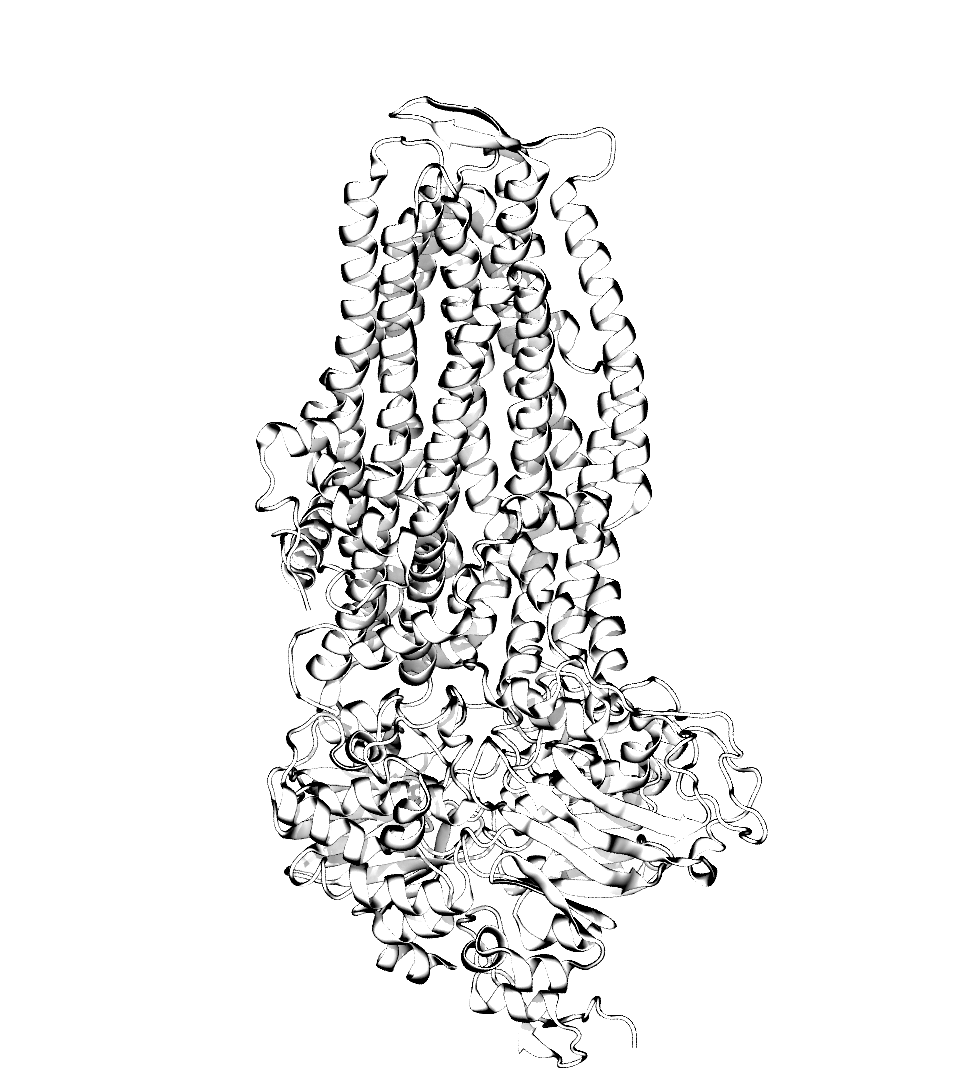
\includegraphics[width=0.8\textwidth]{figures/skeleton_bw.png}
%\vspace{0.1in}
%TO\\
%\vspace{0.1in}
%THE
%{\Large F}ACULTY OF {\Large S}CIENCE\\
\vspace{-0.05in}

\textit{A thesis submitted in fulfilment of the}\\
\textit{requirements for the degree of}

%IN PARTIAL FULFILMENT OF THE REQUIREMENTS\\
%FOR THE DEGREE OF \\
%{\Large D}OCTOR OF {\Large P}HILOSOPHY\\
%IN THE SUBJECT OF \\
%{\Large B}IOPHYSICS\\
\vspace{0.1in}

%\begin{large}
Doctor of Philosophy
%\end{large}

\vspace{0.1in}

%\begin{large}
The School of Physics\\
Faculty of Science\\
The University of Sydney\\
2022
%\vspace{0.05in}
%\end{large}

%\vspace{0.05in}
\end{large}

\end{center}
\end{titlepage}

%=======================================================================================%
\newpage
\begin{center}
Declaration of Original contribution

\vspace{0.5in}

of the dissertation submitted by

\vspace{0.25in}

Miro Alexander Astore

\end{center}

\vspace{0.5in}

\noindent This is to certify that to the best of my knowledge, the content of this 
thesis is my own work. This thesis has not been submitted for any degree or other 
purposes.

\noindent I certify that the intellectual content of this thesis is the product of 
my own work and that all the assistance received in preparing this thesis and sources 
have been acknowledged.

\vspace{1in}

% \begin{tikzpicture}[remember picture,overlay]
%     \node[xshift=4cm,yshift=-14.0cm,anchor=north west] at (current page.north west){%
%     \includegraphics[width=35mm]{Figures/signature-JS.jpg}};
% \end{tikzpicture}

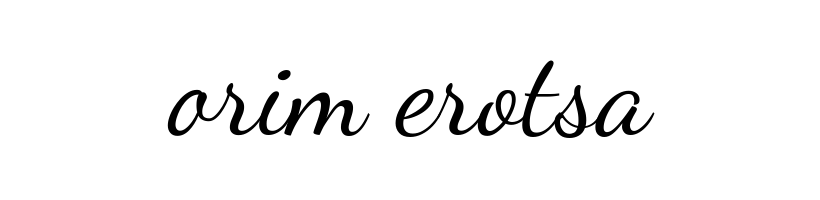
\includegraphics[width=6cm]{figures/signatures/orim_sig_fake.png} \hspace{3.0cm} 09/09/2022\\
% \hspace{12cm} {\large 15/03/2019} \\
\noindent \line(1,0){225} \hspace{1.0cm} \line(1,0){140} \\
 {\em Miro Alexander Astore}, Author \hspace{3.65cm} Date
%=======================================================================================%

%=======================================================================================%
\begin{abstract}
\setcounter{page}{3}
\thispagestyle{plain}

Cystic Fibrosis is the most common fatal genetic condition in Caucasian populations. It is a debilitating disease, significantly shortening the life span of patients and degrading their quality of life. It is caused by deleterious mutations to a protein known as the Cystic Fibrosis Transmembrane conductance Regulator (CFTR). This protein acts as an anion channel.

Over the last decade there have been an increasing number of clinically approved small molecule drugs which act directly on CFTR in order to restore its function. These drugs are called CFTR modulators. Unfortunately, since CF is a rare disease and there are more than 400 mutations which cause it, it is currently unclear which mutations will respond to modulator therapy. This leaves many patients with under studied mutations unable to access modulator therapy.

In this work we performed extensive molecular dynamics (MD) and free energy calculations in order to characterise the many different ways that the CFTR can misfunction. This was done in close collaboration with \textit{in vitro} and clinical experiments in order to understand what types of molecular defects may be treated by existing medications. This work will help more patients access modulator therapy.

We found that rare CFTR mutations exhibit a wide range of molecular defects and that these defects appear to respond to these modulator drugs. The combination of MD, a basic biophysical technique with wet lab studies signals the increasing capability of quantitative physical techniques in biological research.
\end{abstract}

%=======================================================================================%
\newpage


\thispagestyle{empty}


\begin{center}
	\vspace*{\fill}
\textit {In loving memory of Madeline Jennifer Dell} \\
	\vspace*{\fill}
\end{center}
\chapquote{``Fear cuts deeper than swords."}{Arya Stark}

\clearpage

\begin{center}
\begin{Large}
\begin{bfseries}
Acknowledgments
\end{bfseries}
\end{Large}
\end{center}
 Daniel Golestan, a wise man, once told me that to be given the opportunity to create this thesis was a gift. It was. It was a gift given to me by every friend, colleague, teacher, mentor and family member I've spent any time with. The list that follows of those to thank is not complete. If it was you'd be reading about a conversation I had with a middle aged public servant in a hostel north of San Francisco, but that has little to do with Cystic Fibrosis. 

To my parents raised me with not only academic rigor in mind but also a respect for aesthetics which has served me strangely well. I've never had a talent for the creative side of things compared to quantitative disciplines. But were it not for their demand for respect for the arts I'd have remained illiterate. 

To Jeffry for his tutelage and patience, even from across the pacific ocean. 

To Poker. I am a better human being in every conceivable way for having known you. Your wisdom, intelligence and kindness are boundless. You have taught me an inordinate number of things. And yes, I do mean inordinate. 

Nono and Nona I don't think you'll ever read this. I'm sad that you won't understand what I've done but I think you'd be proud if you did. Living in Condell park did more for me than you could know. Far from war torn Beirut or dirt poor Orria I'm sitting in a well lit office writing this with a full stomach and few worries. Sometimes this luck makes my head spin. 

To the whole Waters lab and Shafagh Waters in particular. For your vision, your drive and all your advice. You brought me a truly fascinating PhD project and I benefited greatly from your mentorship. Bridging the gap between cell biology and molecular physics is something that will happen more in the future and I'm lucky to have met such a driven lab to teach me to do so. 

To Serdar, a brilliant mind and a patient boss. Thank you for giving me the best possible experience at grad school I could have asked for. Your willingness to let me pursue self directed projects with a guided hand is a privilege during a PhD and I'm all the better for having gotten it from one of the best. I'm excited to carry some of your physical insight into biological systems to future research projects. 

Maddy, I miss you every day. You couldn't have imagined what it was like to do this after losing you. I carry much of you with me and I wish I had more. I miss your intelligence, your warmth and your love.

You're all in my Loop and I hope I'm in yours.

%=======================================================================================%

%=======================================================================================%
\newpage

\vspace{3in}

\begin{center}
\begin{Large}
\begin{bfseries}
Permission for the Inclusion of Published Work
\end{bfseries}
\end{Large}
\end{center}

\vspace{0.3in}
%The contents of the following chapters are published. \\
%\hspace{\parindent}MA - Miro Alexander Astore \\
%\hspace{\parindent} SK - Serdar Kuyucak \\


\begin{center}
	
\includegraphics [width=\textwidth]{figures/shafa_letter_inclusion_of_published_work.pdf}
\end{center}

\newpage
\begin{center}
\begin{Large}
\begin{bfseries}
Publication Authorship Attribution
\end{bfseries}
\end{Large}
\end{center}

\vspace{0.3in}
\noindent In addition to the statements above, in cases where I am not the 
corresponding author of a published item, permission to include the published 
material has been granted by the corresponding author.

\vspace{1.in}

% \begin{tikzpicture}[remember picture,overlay]
%     \node[xshift=4cm,yshift=-9.0cm,anchor=north west] at (current page.north west){%
%     \includegraphics[width=35mm]{Figures/signature-JS.jpg}};
% \end{tikzpicture}

% \hspace{12cm} {\large 15/03/2019} \\

\includegraphics[width=6cm]{figures/miro_signature.png} \hspace{3.0cm} 09/09/2022\\
\noindent \line(1,0){225} \hspace{1.0cm} \line(1,0){140} \\
 {\em Miro Alexander Astore}, Student \hspace{3.65cm} Date
 
 \vspace{1in}

\noindent As the supervisor for the candidature upon which this thesis is based, 
I can confirm that the authorship attribution statements above are correct.

\vspace{1in}

% \begin{tikzpicture}[remember picture,overlay]
%     \node[xshift=3.5cm,yshift=-19cm,anchor=north west] at (current page.north west){%
%     \includegraphics[width=60mm]{Figures/signature-SK.jpg}};
% \end{tikzpicture}

% \hspace{12cm} {\large 15/03/2019} \\

\includegraphics[width=6cm]{figures/serdar_signature.png} \hspace{3.0cm} 09/09/2022\\
\noindent \line(1,0){225} \hspace{1.0cm} \line(1,0){140} \\
{\em Serdar Kuyucak}, Supervisor \hspace{5.7cm} Date
%=======================================================================================%


%%%%%%%%%%%%%%%%%%%%%%%
%% TABLE OF CONTENTS %%
%%%%%%%%%%%%%%%%%%%%%%%
{
\hypersetup{linkcolor=black}
\tableofcontents
}

\newpage
\phantomsection

\addcontentsline{toc}{chapter}{List of Abbreviations}
%=======================================================================================%
\chapter*{List of Abbreviations}
\label{chap:abbrev}

\begin{center}
\begin{bfseries}
\newcommand\nomenclature[2]{#1 & #2 \\}
\begin{longtable}{@{}p{3cm}@{}p{\dimexpr\textwidth-1cm\relax}@{}}
\nomenclature{${\small AMBER}$}    {Assisted Model Building with Energy Refinement}
\nomenclature{${\small ABC transporter}$}  {ATP-Binding Cassette transporter}
\nomenclature{${\small ATP}$}      {Adenosine Tri-Phosphate}
\nomenclature{${\small BAR}$}      {Bennett-Acceptance-Ratio}
\nomenclature{${\small CF}$}        {Cystic Fibrosis}
\nomenclature{${\small CFTR}$}      {Cystic Fibrosis Transmembrane Conductance Regulator, also abbreviated ABCC7}
\nomenclature{${\small CHARMM}$}   {Chemistry at Harvard Macromolecular Mechanics}
\nomenclature{${\small CMAP}$}     {energy grid correction map}
\nomenclature{${\small COM}$}      {Centre of Mass}
\nomenclature{${\small Cryo-EM}$}  {Cryogenic Electron Microscopy}
\nomenclature{${\small CV}$}       {Collective Variable}
\nomenclature{${\small DMSO}$}     {Dimethyl Sulfoxide}
\nomenclature{${\small DNA}$}     {Deoxyribose Nucleic Acid}
\nomenclature{${\small FEP}$}      {Free-Energy Perturbation}
\nomenclature{${\small FEV1\%}$}   {Forced Expiratory Volume in 1 second}
\nomenclature{${\small FES\%}$}    {Free Energy Surface}
\nomenclature{${\small FIS}$}      {Forskolin-Induced Swelling}
\nomenclature{${\small gA}$}       {Gramicidin A Ion Channel}
\nomenclature{${\small GROMACS}$}  {GROningen MAchine for Chemical Simulations - MD program}
\nomenclature{${\small GROMOS}$}   {GROningen MOlecular Simulation - MD program}
\nomenclature{${\small iPCR}$}     {inverse Polymerase Chain Reaction}
\nomenclature{${\small iPSCs}$}    {induced Pluripotent Stem Cells}
\nomenclature{${\small LJ}$}       {Lenard-Jones}
\nomenclature{${\small MBAR}$}     {Multistate Bennett-Acceptance-Ratio}
\nomenclature{${\small MD}$}       {Molecular Dynamics}
\nomenclature{${\small MM}$}       {Molecular Mechanics}
\nomenclature{${\small MetaD}$}    {Metadynamics}
\nomenclature{${\small WT-MetaD}$} {Well-Tempered Metadynamics}
\nomenclature{${\small NAMD}$}     {Nanoscale Molecular Dynamics - MD Program}
\nomenclature{${\small NBD}$}      {Nucleotide Binding Domain}
\nomenclature{${\small NPT}$}      {Constant Number of particles, Pressure and Temperature. Isothermal-Isobaric Ensemble}
\nomenclature{${\small NVE}$}      {Constant Number of particles, Volume and Energy. Microcanonical Ensemble}
\nomenclature{${\small NVT}$}      {Constant Number of particles, Volume and Temperature. Canonical Ensemble}
\nomenclature{${\small OpenMM}$}   {Open Molecular Mechanics - MD Program}
\nomenclature{${\small OPES}$}     {On the fly Probability Enhanced Sampling}
\nomenclature{${\small OPLS}$}     {Optimised Potentials for Liquid Simulations}
\nomenclature{${\small PBC}$}      {Periodic Boundary Condition}
\nomenclature{${\small PCA}$}      {Principal Component Analysis}
\nomenclature{${\small PDB}$}      {Protein Data Bank}
\nomenclature{${\small PGP}$}      {P-Plyco Protein, also abbreviated ABCB1}
\nomenclature{${\small PI}$}       {Pancreatic Insufficient}
\nomenclature{${\small PKA}$}      {Protein Kinase A}
\nomenclature{${\small PMF}$}      {Potential of Mean Force}
\nomenclature{${\small PME}$}      {Particle Mesh Ewald - Long-range Electrostatics Method}
\nomenclature{${\small POPC}$}     {1-palmitoyl-2-oleoyl-sn-glycero-3-phosphocholine. The most common lipid used in molecular dynamics simulations of eukaryotic cells.}
\nomenclature{${\small RAVE}$}     {Reweighted Autoencoded Variational bayes for Enhanced samplin}
\nomenclature{${\small RMSD}$}     {Root-Mean-Square Deviation}
\nomenclature{${\small RC}$}       {Reaction Coordinate}
\nomenclature{${\small TICA}$}     {Time-lagged Independent Component Analysis}
\nomenclature{${\small TMD}$}     {Transmembrane Domain}
\nomenclature{${\small TMH}$}     {Transmembrane helix}
\nomenclature{${\small US}$}       {Umbrella Sampling}
\nomenclature{${\small VAC}$}      {Variational Approach to Conformational dynamics}
\nomenclature{${\small VMD}$}      {Visual Molecular Dynamics - MD Visualisation Program}
\nomenclature{${\small VUS}$}      {Variants of Unknown Significance}
\nomenclature{${\small WHAM}$}     {Weighted Histogram Analysis Method}
\end{longtable}
\end{bfseries}
\end{center}


\newpage
\phantomsection
\addcontentsline{toc}{chapter}{List of Figures}
{
\hypersetup{linkcolor=black}
\listoffigures
}

\newpage
\phantomsection
\addcontentsline{toc}{chapter}{List of Tables}
{
\hypersetup{linkcolor=black}
\color{black}
\listoftables
}
\clearpage

\clearpage
\thispagestyle{empty}
\vspace*{2.0in}
%\chapquote{``Research is what I'm doing when I don't know what I'm doing."}{Wernher von Braun}

\clearpage
\blankpage

%%%%%%%%%%%%%%%%%%%%%%%
%% MAIN TEXT         %%
%%%%%%%%%%%%%%%%%%%%%%%
%=======================================================================================%
\pagenumbering{arabic}
\chapter{Introduction}
\setcounter{page}{1}
\label{chap:intro}
\chapquote{Whatever complexity means, most people agree that biological systems have it. -Frauenfelder and Wolynes\ref{frauenfelder1994} } {}

\section{Physics in a test tube}
\chapquote{}{}

\vskip 0.5cm

Why can't I  write down an equation will tell me how long I will live? Or how many hairs I will grow?

This might seem like an inane question but if you asked a physicist for the formula for how long it takes a radioactive material to decay or how long it will take an object to fall into a black hole they will be able to answer easily.

What makes the first set of questions so much more difficult to answer?

I posit that it is the diversity of components that makes biological questions so difficult to ask and answer. Biology distinguishes itself amongst scientific disciplines requiring the study of systems that are both complex and heterogeneous. In the study of more simple physical systems a simple analogy such as a mass on a spring or a gas of hard spheres can be extremely successful in explaining macroscopic phenomena. For biological systems there appears to be too much complexity for such analogies to have the same level of success. They may struggle to answer questions such as "If this gene mutates how will that affect lung function?" "If this drug were given at a higher dosage what would its effect be?" "What if we change this chemical moiety?" At the moment, a trained chemist needs to go and answer these questions pipette in hand, the physicist with their notebook is hopeless.

It seems like a silly question but it seems important to ask why we can't just use a device similar to a harmonic oscillator or a perfect black body to speculate at useful answers for these quantitative questions. The answer is just as silly. If you look with your naked eye at your arm, you will notice hair, pores, dry skin, dead skin, perhaps even tendons and muscles under the skin. If you take a microscope you will notice the 3 layers to your skin with different functions and composition. If you were to take a single cell from any of those layers and stain it to distinguish features in an electron microscope you would notice all sorts of complex structures and the size and number of these structures would vary depending on where you took the cell from in the body. Within and between each those structures is a salty, wet dance of molecules large and small. This heterogeneity on length scales hints at the reasons behind biology's physical complexity. Plasma physics is often characterised by the density of the plasma studied. This parameter may span 28 orders of magnitude from a dense stellar core to the sparse intergalactic nebulae. The same mathematical tools can be used to map any plasma in these energy scales. Would that we were so lucky in biology. We struggle to apply same physical models to deal with phenomena across a single order of magnitude.  


Thus, in order to move towards more predictive theories of biology it is necessary to consider much more of the fundamental physical processes occurring within biological systems than simply searching for statistical trends. One form of this from fundamentals approach is the simulation of every atom in a biological system. Although computationally expensive, this approach appears necessary due to the heterogeneous nature of biological systems. 

One of the things we're trying to do with molecular dynamics is fill in the gap left by the sequence->function paradigm which is internalised in current understandings of molecular biology. We usually talk about how the sequence of the gene defines its function because it gives the protein its structure but really there is a considerably larger amount of regulatory pressure exerted by the environment. This is what is missing from the sequence alone paradigm.

\section{What is Physics?}
Personally I have always given answers along the lines of "the study of the movement of energy within a system" or when I was in high school "The study of how things move". Although adequate for a layman these might obscure the fundamental structure within physics that make it such a powerful tool. It is the conception of some causal unit in a system and the ability to scale up the behaviour of that unit to make predictions about measurable phenomena.

This might take a few different forms at different scales, it's what makes physics feel like the most "fundamental" of the sciences. 

Examples include:

Newton's laws of gravitation to explain the organisation of the solar system. 

Einstein's theories employing Reimannian geometry to track the motions of galaxies and black holes.

The conception of atoms as hard spheres used to derive the macroscopic behaviour of gasses.

The schrodinger wave function to find the structure of atoms, which can then be integrated further up to find their macroscopic organisations. More on this later.

Biological systems exhibit such a problem for the physicist because unlike the above problems it is extremely hard to pick out a fundamental unit to even begin our upwards journey. An evolutionary biologist might say to choose the "gene" but this is actually far too high in our spatial heirarchy already. Really a gene is only meaningful to the dance of life if it has partners to dance with. Genes of hard spheres ?

A coil of DNA in water doesn't really do much in solution except decay without machinary that can preserve, read, translate and replicate it. The gene is an emergent property, we have to go deeper. 

So, what creates the gene? 

A slew of biological machinary that mostly take the form of proteins. These proetins are a special case of chemistry, with many observable functions. Their sequence is  coded by the DNA in something reminiscent of a strange loop \cite{Hoffstadter2008}. 

This self referential loop is one of the reasons biology is so difficult. Since we know that this strange loop is kicked off by atomic interactions we will start there. As we are taking a physical, pragmatic approach here it would make sense to begin with the protein, after all, they stave off the march of entropy constantly trying to eat up all of your cells. It also just so happens that they are much easier to understand computationally since their motions are faster and more flexible. 

The first level sub cellular organisation is perhaps the most intimdating first step for me personally after spending 4 years simulating a single protein. Glimpsing the complexity within a single one of these molecules has been one of the most existential experiences of my life but the knowledge that there are astronomical numbers of these things inside me all of the time 

It is hoped that illustrating the monumental task in both intellectual effort and resources of incrementally increasing the understanding of a single protein amongst tens of thousands will give the reader and understanding of how we might continue our quest to understand the molecular dance that plays within all of us.  
 
This makes sense if we think about it 
Somewhere on the scale between a single protein and a single cell this is what we consider "life". We have single unicellular organisms but we don't have uniproteomic organisms. So the fundamental length scale of life is somewhere between $10^{-10}m$ and $10^{-3}m$. This is the first loop in our strange loop.

After this things start to run away from me with my handful of GPUs and limited patience. So in this thesis we will only discuss single proteins.
%Biological strange loops would not seem to be as self similar as the clean nice logics in the strange loop of the Godelian knot. Why is this?


\section{Ion Channels: Natures laboratories to Teach Us Biophysics}
The physiological importane of ion channels became clear after the experiments of Hodkin and Huxley. These mathematicians took nerves from fished giant squid and measured the current running through the nerve in response to electrical stimulation. What they found was intruiging. Current would only flow when the input signal was of a sufficient voltage. The measurements and modelling they carried out gave an exciting set of results. They found that the cell had to maintain a constant electrochemical gradient, they discovered that the presence of voltage gated ion channels and cation selective ion channels\cite{hodgkin1952}. Each of these features, motivated by mathematical modelling have been found to be critical to the functioning of the cell and fundamental to the foundation of molecular biophysics. The following set coupled ordinary differential equations were discovered by testing functions which fit the measurements taken from the squid axon.   

\begin{equation}
\begin{aligned}
	I = C_m \frac{dV}{dt} &+ \bar{g}_K n^4 (V - V_K) + \bar{g}_{Na} m^3 h (V - V_{Na} ) + \bar{g}_l (V-V_l) ,  \\
	\frac{dn}{dt} &= \alpha_n(V)  (1-n) - \beta_n(V)  n, \\
	\frac{dm}{dt} &= \alpha_m(V)  (1-m) - \beta_m(V)  m, \\ 
	\frac{dh}{dt} &= \alpha_h(V)  (1-h) - \beta_h(V)  h  
\end{aligned}
\end{equation}

The $\alpha$ and $beta$ parameters are the proportion of the sodium and potassium channel populations which are activated, respecitively.  This example shows how basic theoretical tools can be used to predict and discover physical phenemon in biological systems. The Hodkin Huxley model proved the existence of a cell's resting potential, the posibility of voltage gated ion channels, and channels whose pores are selective for certain ions. Even today the molecular mechanisms behind some of these discoveries are debated. In this thesis we aim to do the same by building up from fundamental quantum mechanics in order to understand the motion of single proteins so we might speculate as to the function of the whole organism.

Similar to the above story, ion channels have always motivated the early pioneers of molecular biophysics. This is due to their ubiquity and importance in biological systems and the ease of measuring their activity with biochemical assays. One just needs an oscilloscope to measure their current. As cell biolgoy has advanced it has become clear that the resting potential of a cell is critical to its function, regulating many chemical reactions inside it.


These factors have to allowed biophysicists sufficient data to build sufficiently accurate models of biomolecular systems which generalise to other systems. Leading to a thriving field, analysing systems as diverse as protocells to gold nano particles CITATIONS NEEDED.

The discovery of voltage gated channels and a resting potential .


%=======================================================================================%

\section{Studying Cystic Fibrosis to Learn Biophysics}

The sad truth of this debilitating disease is that those afflicted are extremely unlucky. A single, small change to the genome and their lungs fill with sticky mucus and become infected with bacteria, each breath cumbersome. Personally, I've not met somebody who has this disease. I have consistently wondered what perspective I'm missing by not suffering myself from such a condition or even knowing somebody with it. I'm not been trained in the ethics of studying medicine.

In this way, my motivations for studying this protein aren't solely focussed on treating disease. There is a perspective on protein evolution which states that the primary sequence of a particular gene contributes to the overall fitness of an organisms by a formula. \cite{}


It just so happens that the CFTR gene sits at the precipice of a daunting cliff in sequence space. So by taking small steps in sequence space and plunging down this cliff we can try to understand how we might push the ball back up the cliff and retain functionality.

Moreover, by learning the nuts and bolts of what goes wrong with CFTR we can start to think about where some of these cliffs might be in other places in the proteome, to gain function and avoid disease and debilitation.

The reality of disease pathogenesis being caused by so many different mutations means that there has been decades of investigation into the function of every domain in the protein. 

Due to the array of disease causing mutations which occur accross the cystic fibrosis protein, there is a large body of literature on its unique function. This allows us a glance into its function and an opportunity to simultaneously perform basic biophysical research while directly assisting in furthering patient outcomes.  

\section{Well. We're in the future}
Throughout science, the integration of experimental data with theoretical models leads to new and exciting research, this is particularly true in biology with its important applications. Wet lab biologists take advantage of experimental techniques which allow them to understand the dynamics and structure of living things from the top down. The finer the experimental instrument, the finer the detail they may resolve. Conversely, computational and theoretical biologists take a bottom up approach, we aim to take the granular details of a system, and integrate them upwards to model the macroscopic behaviour of that system. With more powerful computers and more detailed models we can make predictions about the behaviour of more complex systems. What is so exciting about the current era of biological research is that the domains of these two approaches are beginning to overlap, where they can synergize  and drive further breakthroughs. As we discover more systems where this overlap can be found we will cure diseases and create amazing things.

The reason this has happened before in physics is two fold. Physical systems are much more homogeneous. So it's much easier to integrate upwards in length scale. Once you understand the pairwise interaction between two components it's simply a question of having the theoretical and computational capacity to model the bulk behaviour of that system. 

The difference with biological systems is that they have so many different components that finding an analytic or even computationally tractable solution is usually impossible. However, as we collect more data and and build more powerful computers we can approach more complete models. These in turn inform more powerful theoretical models these help direct the material efforts of experimental expertise . 

Alphafold is a good example. This new breakthrough builds on decades of inquiry from the structural biology community and advancements in AI to give high resolution protein structures. Now this result can be used to fill in the gaps of structural biology. Crucually, alphafold konws what it doesn't know. So we can tell where to direct the efforts of structural biology. Together these advances will fill more gaps in our knowledge of protein physics. 

%=======================================================================================%
\chapter{From Protons to Proteins: Methods to simulate the inside of a cell.}
\numberwithin{equation}{chapter}
\label{chap:methods}

\section{Quantum Mechanics is Not Tractable at the Scale of Biology.}
Living things are made of atoms and atoms themselves are composed of many particles. The motions of atoms and their constituent particles are governed by quantum mechanics. Unfortunately, performing simulations for the number of atoms involved in proteins and other cellular components at quantum mechanical accuracy is impossible. Hence, we will show how to take the fundamental formulation of atomic interactions in the Schr\"{o}dinger wave equation and apply approximations in order to produce a model which is capable of simulating macromolecular systems at biologically relevant timescales. 

We will gradually integrate upwards, beginning with the interactions in a single atom we will work our way up to a complex macromolecular system with lipids, water, salts and of course, proteins. Ultimately this section rationalises the treatment of atoms as point charges in classical molecular dynamics simulations. It is hoped that this section can be of use to both biologists and physicists, in order to teach the physicist what they need to know about the models they will be using to perform these simulations (and the many technical problems they will encounter) and to inform the biologist what the physicist is doing with all that computer time. 

\subsection{A full quantum mechanical treatment}
Since we are dealing with atoms which are governed by quantum mechanics we must begin our journey upwards with the time dependent form of the Schr\"{o}dinger wave equation. 

\begin{equation}
i\hbar \frac {\partial}{\partial t} \Psi (\textbf{x},t) = \big[ -\frac{\hbar ^2}{2m}\nabla^2 + V (\textbf{x}, t) \big] \Psi (\textbf{x},t) 
\label {schordinger_time_dependent}
\end{equation}

In quantum systems we treat all particles as waves hence the use of the wave function $\Psi (\textbf{x},t)$. The complex amplitude of the wave function $|\Psi (\textbf {x}, t)|^2$ tells us the likelihood of detecting the particle at time $t$ and at place $\textbf{x}$. The term in the brackets correspond to $-\frac{\hbar ^2}{2m}\nabla^2 $ the kinetic energy of the particle with mass $m$ while $V (\textbf{x}, t)$ is the potential energy of the system. Given that the left hand term $i\hbar \frac {\partial}{\partial t} \Psi (\textbf{x},t)$ contains a gradient with respect to time, it governs how the wave function will evolve in time.

When the external potential $V$ has no explicit dependence on time, this equation reduces to the familiar time independent form. 

\begin{equation}
	E \Psi (\textbf{x}, t) = \big[ -\frac{\hbar ^2}{2m}\nabla^2 + V (\textbf{x}) \big] \Psi (\textbf{x}, t) = H \Psi(\textbf{x}, t) 
 \end{equation}

Note that the wave function $\Psi (\textbf {x}, t)$ is still allowed to evolve in time. 

In an atom there are two types of particles, nuclei which we will denote with the subscript $i$ and electrons denoted by $e$. In order to treat these elements separately we decompose the Hamiltonian of the system into a few components. 

\begin {equation}
H = T_n + T_e + V_{n-n} + V_{n_e} + V_{e-e}
\end {equation}

Where $T_n$ and $T_e$ denote the kinetic energy of the nucleus and electrons respectively. While $V_{n-n}, V_{n-e}, V_{e-e}$ denote the potential energy for interactions between nuclei, between electrons and nuclei and between electrons respectively.

Since the potential terms all describe charged species, they follow Coulomb's law and have the form.

\begin{equation}
	V_{n-n} = \sum_{i>j} \frac{q_e^2 z_i z_j }{|\textbf{R}_i-\textbf{R}_j|},\quad V_{n-e} = \sum_{i,l} \frac{q_e^2 z_i }{|\textbf{r}_l-\textbf{R}_i|},\quad  V_{e-e}  = \sum_{l>k} \frac{q_e^2 }{|\textbf{r}_l-\textbf{r}_k|}
\end{equation}

Here the $z_i$ represent the charge atomic number (and thus the charge) of the $i$th nucleus and $q_e$ is the unit charge of the electron. The reason for the separate coordinates $R_i$ and $r_l$ is to separate out the treatment of nuclei and electrons which will be important once we apply the Born-Oppenheimer approximation.

Meanwhile, the kinetic energy terms are quite simple. 

\begin {equation}
T_n = - \sum_i \frac{\hbar^2}{2M_i} \nabla_i ^2,\quad  T_e = - \sum_l \frac{\hbar^2}{2m_l} \nabla_l ^2
\end {equation}

$M_i$ represents the mass of the $i$th nucleon and $m_l$ represents the mass of the $l$th electron. The separate subscripts $i$ and $l$ are due to the different coordinates which we use to denote the positions of the nuclei and the electrons. The reason for this will become clear when we apply the Born-Oppenheimer approximation to separate the wave functions and solve them separately.

Here, the $M_i$ are the masses of the nuclei and the operator $\nabla^2 = \frac{\partial^2}{\partial x^2} + \frac{\partial^2 }{\partial y^2} + \frac{\partial^2}{\partial z^2} $


\subsection{The Born-Oppenheimer approximation.}
We now make use of the Born-Oppenheimer approximation \cite{Born1927}. This is motivated by the observation that electrons are 3-4 orders of magnitude lighter than the nucleus, and so we can assume that the electrons will respond instantaneously to any changes in the wave function of the nucleus. Thus, we can disregard $T_e$, $U_{n-e}$ and $U_{e-e}$ 

%In the case of hydrogen we lose an order of magnitude so the approximation is less valid, especially at room temperature. CITATION NEEDED

This allows us to split the total wave function into two parts using a direct product. One term deals with the nuclei and one with the electrons in the system. 

\begin {equation}
\Psi(R_i,t) = \psi_e (r_l,R_i) \psi_n(R_i,t)
\end {equation}

\section{Classical MD, Molecular Motions Without Quantum Mechanics}
The Born-Oppenheimer approximation gives rise to Hartree-Fock methods which allow calculations of the organisation of electron clouds around small molecules. This lets us derive the energy profile of certain degrees of freedom within the molecule such as the energetics of stretching out a bond or twisting a dihedral angle. 

However, even with these approximations simulating a large number of atoms is not computationally tractable. So, we must use another round of approximations to reach the spatial and time scales necessary to simulate biological molecules. We do this by creating a set of mathematical functions the calculations further. Here we use a set of virtual springs and other simple models for the energetic interactions between atoms. This creates what's known as an effective potential. So named because it effectively approximates the behaviour of the full quantum mechanical system.

This formulation gives us classical molecular dynamics sometimes referred to as molecular mechanics. The aim of the classical forcefields discussed here is to use \textit {ab initio} MD as a target to approximate. 

The CHARMM effective potential employed in this work is common in all-atom molecular dynamics. The same  functional forms are used in other forcefields such as AMBER, GROMOS and OPLS but with different parameters and design philosophies. [CITATION NEEDED]

We split up the molecular potential into several components dealing with the energies from covalent bonds, including bond stretching, twisting and pinching. As well as energies associated with the forces that atoms exert on each other when they are not bonded together. Namely and Coulomb forces due to electric charges on the atom and attractive Van Der Walls interactions and repulsion due to Pauli Exclusion the latter two forces are combined into one term we will analyse in detail $U_{LJ}$.

\begin{equation}
	U_{CHARMM} = \underbrace{U_{LJ} + U_{Coulomb}}_{U_{non-bonded}} + \underbrace{U_{bonds} + U_{angles} + U_{dihedrals} + U_{impropers}}_{U_{bonded} }
	\label{CHARMM}
\end{equation}

Interestingly, the bonded terms may all reasonably be approximated by harmonic springs. 

\begin{equation}\label{bonded_eqs}
	\begin{aligned}
	U_{bonded} = \sum_{bonds} k_{b} (b-b_0)^2 + \sum_{angles} k_\theta(\theta-\theta_0)^2+ \sum_{Urey-Bradley} k_u(r_{UB}-r_{UB_0})^2   \\ + \sum_{dihedrals} k_\phi (1+\cos(n \psi - \delta)) + \sum_{improper-dihedrals}  k_{\phi} (\phi - \phi_0)^2 
\end{aligned}
\end{equation}

Here, the $k_i$ terms correspond to the strength of the harmonic restraint for that parameter. The $0$ subscript denotes the equilibrium position for that parameter. Even though this formulation is quite simple, it has empirically been shown to accurately model the quantum energetics of bonded interactions at room temperature this can be seen in figure \ref{morse_potential}.

\begin{figure}
	\begin{center}
	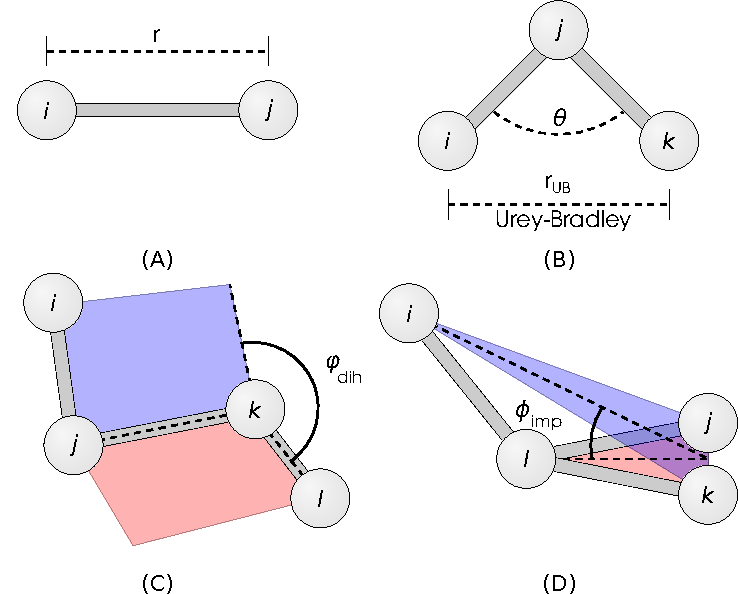
\includegraphics[width=10cm]{figures/bonded_interactions.pdf}
	\end{center}
	\captionsetup{singlelinecheck = false, justification=raggedright}
	\caption[The Bonded Interactions Calculated In Classical Forcefields]{\textbf{The Bonded Interactions Approximated In Classical Forcefields.}}{
		(A) The energy of Bond Stretching is approximated as a harmonic oscillator with respect to their separation $r$. (B) Angles between neighbouring covalently bonded atoms are also approximated as a harmonic oscillator with respect to the angle $\theta$. In some forcefields such as CHARMM there is a correction term for these angular interactions known as Urey Bradley forces. This is calculated using the separation between the non-bonded atoms $i$-$k$ in the triplet with the parameter $r_{UB}$. (C) The dihedral angle between four atoms is calculated by constructing two planes. Each plane is constructed to contains three of the four atoms in the set. One plane encompasses atoms i, j and k here  colored in blue and the other plane contains the j, k and l atoms colored in red. The dihedral angle is then calculated by taking the angle between these two planes along the line they intersect, the line formed by the j-k bond. (D) The improper dihedral angles are again calculated with the use of two planes. Containing i, j and k and j, k and l respectively. The difference is that this parameter parametrises planarity of a molecular configuration rather than the flexibility of torsion angles.
	}
	\label{charmm_bonded}
\end{figure}


In classical forcefields the non-bonded interactions are expressed using the Couloumb's law because the partial charges assigned to each atom and the Lennard-Jones potential to approximate the interactions arising from both Pauli exclusion and Van Der Walls Interactions.


\begin{equation}\label{nonbonded_eqs}
	\begin{aligned}
		U_{non-bonded} = \underbrace{\sum_{i>j} \epsilon_{ij} \Big( \Big(\frac{\sigma_{ij}}{r_{ij}}\Big)^{12} - \Big(\frac{\sigma_{ij}}{r_{ij}}\Big)^{6} \Big)}_{U_{Lennard-Jones}} - \underbrace{\sum_{i>j} \frac{q_i q_j } {r_{ij}}}_{U_{coloumb}}
	\end{aligned}
\end{equation}


The $\sigma$ parameter denotes the location of the local minima in the Lennard-Jones potential. This is the optimum distance that two atoms will rest against each other in the absence of other effects. The $\epsilon$ parameter denotes the depth of the potential well, or how stable the two atoms will be in the minimum energy configuration. This is very important for certain physical parameters such as osmotic pressure  \cite{Yoo2018}

Conversely, the partial charges in a system have the greatest influence on the solvation energy.

By focussing on these two physical parameters we can isolate and improve the non-bonded parameters.

\begin{figure}
	\begin{center}
	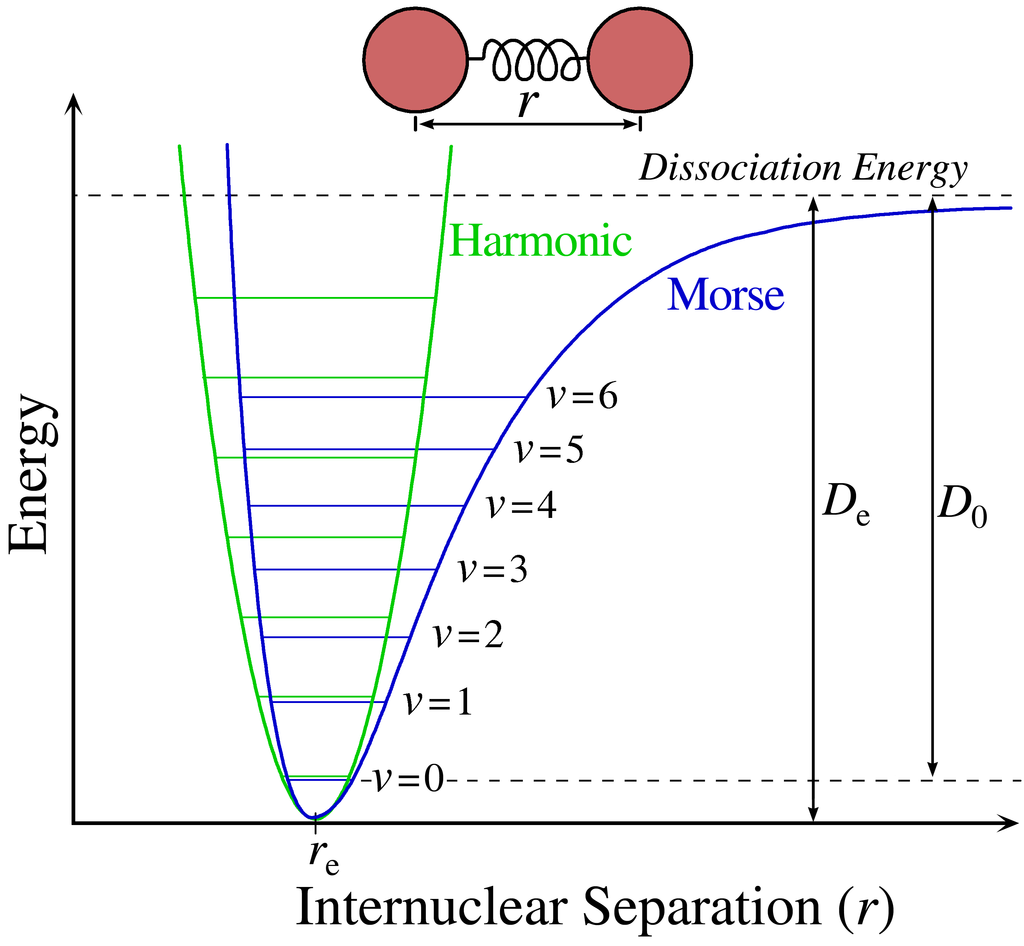
\includegraphics[width=7cm]{figures/Morse-Potential.png}
	\end{center}
	\captionsetup{singlelinecheck = false, justification=raggedright}
	\caption[The Morse Potential Compared to a Harmonic Potential] {\textbf{The Morse Potential Compared to a Harmonic Potential}}{
		The Morse potential was formulated to approximate the potential the potential energy surface of the separation of covalent bonds (blue). At low temperatures (the ground state, v=0) like those found in classical MD there is good agreement between the Morse potential and the harmonic oscillator (green). Credit Mark Somoza 2006. 
}
	\label{morse_potential}
\end{figure}

\subsection{Philosophy of Different Molecular Mechanics forcefields.}
At the time of writing, the four popular forcefields for the simulation of biomolecules are: AMBER, CHARMM, GROMOS and OPLS. Each of these have a slightly different philosophy in their formulation. They may be bottom up, as in the case of AMBER and CHARMM or top down, in the case of GROMOS and OPLS. Bottom up forcefields take the results from quantum \textit{ab initio} calculations and approximate them with the functional form mentioned above. Conversely, top down forcefields take experimental measurable such as Osmotic pressure, solvation energy. This philosophy is closest to physics 

\subsection{The Process of Preparing a Simulation}
The process of taking a molecular structure and putting it in a cellular environment to simulate it at physiological temperatures is both an art and a science. It's a science because a biophysicist must be aware of the many tricks that structural biologists use to image a macromolecular complex. But it's an art because accounting for those tricks and modifications is rarely straight forward. How do you build a missing loop? What charge state is an amino acid most likely to take during the physiological context.

\subsection{Controlling the Temperature and Pressure in a Simulation}

\subsection{Periodic Boundaries to Simulate a Realistic System Size}


\subsection{Short Comings of Classical MD}
The short comings of classical molecular dynamics fall into two classes whose solutions stand opposed to one another. These are the accuracy of the chemical forcefields outlined above and the inability of modern computers to deliver enough samples of the energy landscape to collect sufficient statistics for rigorous conclusions. The issue is that, as the above physical formulation might indicate. The more accurate the forcefields, the more computationally expensive. And so the solutions to the two are constantly in tension with one another. In the next section we will explore the current efforts to bring solutions.

\subsubsection{The Problem with Forcefields}
These approximations are not without a cost to accuracy. In certain situations, many of which are biologically relevant, it has been shown that quantum effects such as polarisation play an important role in the dynamics of the system. This has been demonstrated in the literature for Gramicidin where polarisable forcefields are able to more accurately reproduce the experimental results of current.

The other context where polarisation is important to consider are on divalent ions. Here, the solvation energy is underestimated due to the consistent lack of polarisation, making investigations of these biologically important chemical species difficult.

However, for most situations, particularly those involving bulk water and protein motions Molecular Dynamics is proving to be an invaluable tool for investigating the properties of biological systems CITATION NEEDED. Sadly, it should be kept in mind that classical MD is not able to simulate any chemistry such as forming and breaking or the change a change in profanation state. Such interactions require considerations of Quantum Mechanics which are computationally expensive.

There are several efforts to correct address some of the above issues. These include the inclusion of the effects of polarisation, the most popular methods at the moment being adding a massless drude oscillator as an extra bead to most(?) atoms as in the CHARMM drude forcefields, championed by the Mackerell lab and the use of forcefields such as AMOEBA which explicitly calculate the dipole and quadrupole moments of each atom. These both substantially increase computational cost but have displayed much better agreement with experiments in biological systems where classical forcefields have been shown to fail \cite{ngo2021}. 

Ultimately, the functional form in equation \ref{CHARMM} does not have sufficient degrees of freedom to address all possible chemical contexts  and so careful consideration must always be given to whether the forcefield is being used in a faithful way to what it was intended to simulate. So long as the user is aware of the situations where classical forcefields fall short they can be a powerful tool for the study of molecular systems.

\subsubsection{The Problem with Sampling}

To physicists the sampling is the more intuitive. Collecting sufficient statistics about the system of interest is difficult and comes at both a computational and human cost. Even though computers have sped up exponentially for the last 50 years we are still orders of magnitude from being able to reach the time scales of many biological processes. As is we struggle to sample the time scales of diffusion through an ion channel, despite the problem standing for decades. 

The slow time step demanded in classical MD due to the fast motions of certain atomic groups such as hydrogen is fundamentally at odds with the time scales of many important biological processes such as drug binding or protein folding which occur on the time scale of  milliseconds or seconds. 

Methods are now emerging which intelligently drive the simulation toward regions unexplored in the collective variable space by unbiased simulations. For some time the field has used steered methods or adaptive sampling methods such as Umbrella Sampling or Metadynamics to drive the simulation toward sections of the energy landscape which are under sampled. These methods universally rely on a choice of collective variable which closely corresponds to a slow degree of freedom. Such a choice is not usually simple. In the case of ion channels one may rationally choose the placement of the ion along the conduction pathway as the collective variable but the choice is less obvious in the case of more global conformational changes.

The advances we are seeing at the moment which I find exciting are the use of machine learning methods to tease out these degrees of freedom in order toaccelerate them with already established free energy methods. These have the potential to uncover new drug binding pockets and revolutionise our understanding of biomolecular systems. 


\subsection{Accelerating Simulations with Virtual Site Topologies}
The discrete time step, $\Delta t$ in equation \ref{verlet}, is one of the most important determinants in the performance of the simulation. We would like $\Delta t$ to be as large as possible, so that the minimum number of calculations are made to sample the desired time scale, which usually runs to nanoseconds or milliseconds.  

Due to Nyquist's theorem the $\Delta t$ parameter must be less than half the speed of the fastest degree of freedom in the system CITATION NEEDED. In the case of biomolecular systems we are challenged by the fact that they are so hydrogen-rich. Since hydrogen is so light, its motion is much faster compared to the other molecular motions involving heavier, slower moving atoms. Its correlation time is on the order of 1 femtosecond, in classical simulations we are able to get away with using 2 femtoseonds by enforcing a rigid hydrogen bond length, i.e interpolating its position backward from the 2 fs timestep.  

However, there are more involved strategies to account for these effects. Hydrogen Mass repartitioning and multiple time stepping have become popular but we will discuss Virtual Sites in detail as they were used for some simulations in this thesis.  

\begin{table}
	\begin{center}   
		\begin{tabular}{ |c|c|c|}
			\hline
			Motion & Timescale \\
			\hline
			Covalent Bond-stretching & $1-2\times10^{-15}\text{s}$ \\
			Covalent Bond-angle bending & $5-10\times10^{-15}$s \\ 
			Sidechain  Motions & $1 \times10 ^{-12}\text{s}-1\times{10^-6}s$ \\
			Rigid Body Motions (depending on size of body) & $1 \times10 ^{-9}\text{s}-1s$ \\
			Ion Conduction & $1\times10^{-9}\text{s}-10^{-6}$ \\
			Protein Conformational Changes & $1\times10^{-9}\text{s}-10^{-3}$ \\
			Alpha Helix Formation & $1\times10^{-9}\text{s}-10^{-6}$ \\
			Beta Sheet Formation & $1\times10^{-6}\text{s}-10^{-3}$ \\
			Protein Folding & $1\times10^{-6}\text{s}-10\text{s}$ \\
			\hline
		\end{tabular}
\end{center}
%\begin{tabular} { |c|c|c| } 
%	\hline
%	%\label{atomic_motions_speed}
%	System Description & Fastest Degree of Freedom & Characteristic Timescale \\ 
%	\hline
%	Uncoupled Atoms  & Atom Translation & 10 fs  \\ 
%	Rigid Molecules & Rigid Body Rotation & 5 fs \\  
%	Flex. Molecule with Rigid Bonds & Bond Angle Vibrations & 2 fs  \\ 
%	 Flex. Molecule with Flex. Bonds & Bond Stretching Vibrations & 1 fs  \\ 
%	\hline
%\end{tabular}
	\captionsetup{singlelinecheck = false, justification=raggedright}
	\caption[Timescales of Motions in a Molecular System]{\textbf{Timescales of Motions in a Molecular System}} {The time step of a simulation must be small enough to capture the motions in the fastest degree of freedom. In hydrogen-rich biomolecular systems the bottle neck can be found in the fast bond vibrations in lighter atoms. This stands in tension with the phenomena we are interested in on longer timescales such as protein folding. Sources: \cite{schlick2010}\cite{brooks1988}\cite{flood2019}\cite{werner2012}}
\end{table}

As you can see in table \ref{atomic_motions_speed} the fastest motion in molecular systems is dictated by the translation of hydrogen atoms. Virtual site topologies aim to remove the requirement for calculating these motions every time step by instead interpolating the positions of hydrogen atoms from the positions of surrounding heavy atoms. This follows from the 3600cm$^{-1}$ peak in the resonance infrared resonance spectrum of biomolecules corresponding to the bond stretching oscillation of the H-O bond. \cite{schlick2010} Setting the time step of simluations to 1/10th of this period gives sufficient gives the Verlet integrator sufficient resolution to capture the motion and maintain the stability of the energy function.

\section{Free Energy Calculations: Making Simluations More Useful}
The above work sets out how to perform unbiased MD simulations. These are powerful tools but as mentioned in section \nameref{sampling_problem} if one only relies on unbiased simulations they will quickly exceed the available computer power. So we must be clever in how we direct our available resources. This means intelligently sampling sections of the molecular phase space which are of interest to us physically but are not reached in our unbiased simulations. A technique that is used extensively throughout this thesis is the addition of a biased potential to the molecular potential $U_{MM}$ calculated for the purposes of unbiased simulations. This will drive the simulation to regions of interest. 

\begin{equation}
U_{FEC}  = U_{MM} + U_{biased} (\xi)
\end{equation}

Note how the $U_{biased}$ term is explicitly dependent on a parameter $\xi$. This parameter is known by many names, an order parameter, a collective variable or a reaction coordinate. Each of these names 

\subsection{Umbrella Sampling}

\subsubsection{Weighted Histogram Average Method}

\subsection{Metadynamics}


%=======================================================================================%
\chapter{Review of the Molecular Cause of Cystic Fibrosis and Its Treatment}
\label{chap:cftr_review}
\chapquote{Because of what's inside me; Because of my genes;-Bob Flanagan, "Why."}{}
\newpage
%Authors note:
% We begin with a breif overview of the disease Cystic Fibrosis as it is the main motiation for this project. A horrendous disease for which we will soon find a cure.
% The purpose of this chapter is to present an overview of CFTR's structure and mechanism of action as discovered by a combination of structural and physiological studies. In addition to the actions of CFTR modulators.
\section{Clinical outcomes of Cystic Fibrosis}
Cystic Fibrosis (CF) is the most common fatal genetic condition in Caucasian populations. 165 000 people are afflicted globally. Even with decades of research there is no known cure for CF. With the average life expectancy of patients falling below 50 even in countries with developed health care systems such as the USA and Australia\cite{}\cite{}. The cause is from a build up of salts inside epithelial cells. This causes the surface of the epithelium to dehydrate. When dehydrated the cilia on the epithelium collapse leaving them unable to clear the mucus that naturally lines the airway\cite{boucher2007}. The dehydration mentioned earlier causes the mucus to thicken. This buildup has two pathogenic functions. Firstly it inhibits the normal function of the organ, as mucus fills ducts that would normally pass nutrients in the pancreas or absorb gasses in the lungs. Secondly, the stationary mucus allows bacterial infection, this can further degrade lung function and remains one of the most troublesome chronic complications in CF patients. 

Much of the clinical research into CF has been managing the movement of this mucus and the populations of bacterium in it. Patients require hours of physical therapy each day to help clear this mucus since their lungs are unable to. They must also inhale saline solutions in order to counteract the osmotic pressure in their epithelium. This helps draw more moisture out of the epithelial cells to allow the cilia to move. 

CF patients struggle to intake nutrients due to the build up of mucus in the ducts of their pancreas and large intestines. This leads to CF related diabetes which afflicts roughly half of adults with CF \cite{Kayani2018}. Patients with CF related diabetes are often administered enzymes and must adhere to a specific diet. 

\begin{figure}
	\label{CF_life_expectancy}
	\begin{center}
	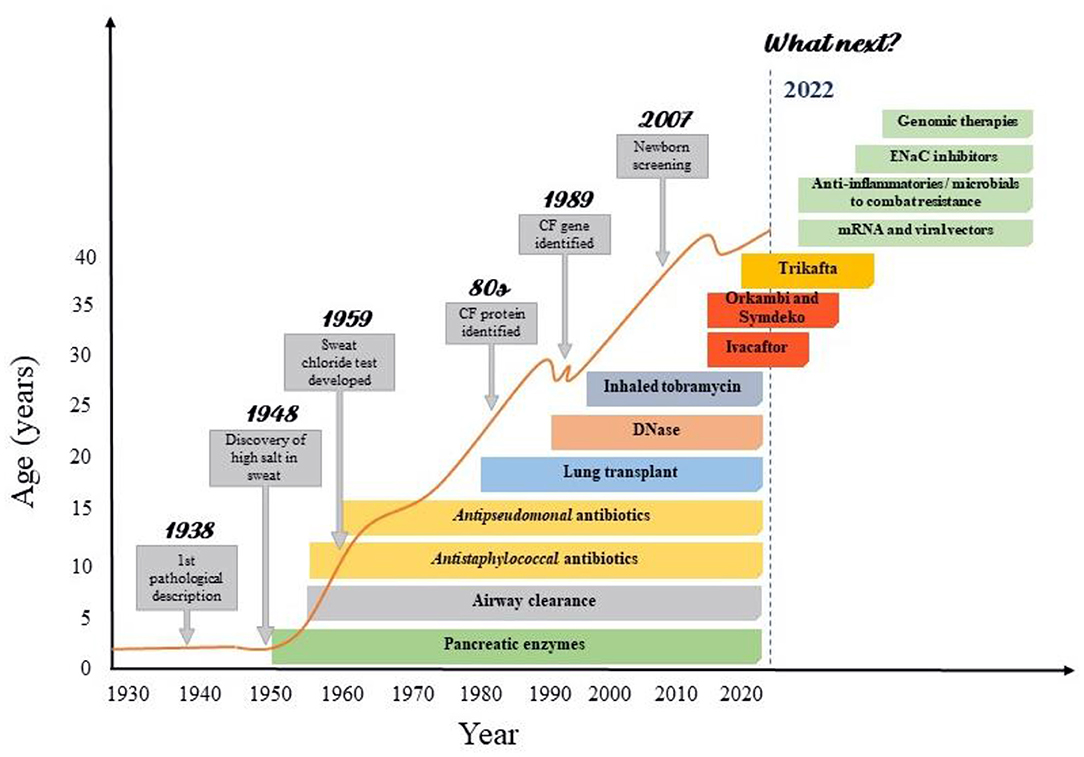
\includegraphics[width=0.6\textwidth]{figures/CF_life_expectancy.png}
	\end{center}
	\captionsetup{singlelinecheck = false, justification=raggedright}
	\caption[CF Clinical Progress] {\textbf{CF Clinical Progress}}{Life expectancy of CF patients correlates highly with translational research. Source \cite{garcia2022}} 
\end{figure}

\section{CFTR Structure}

\begin{figure}
	\begin{center}
	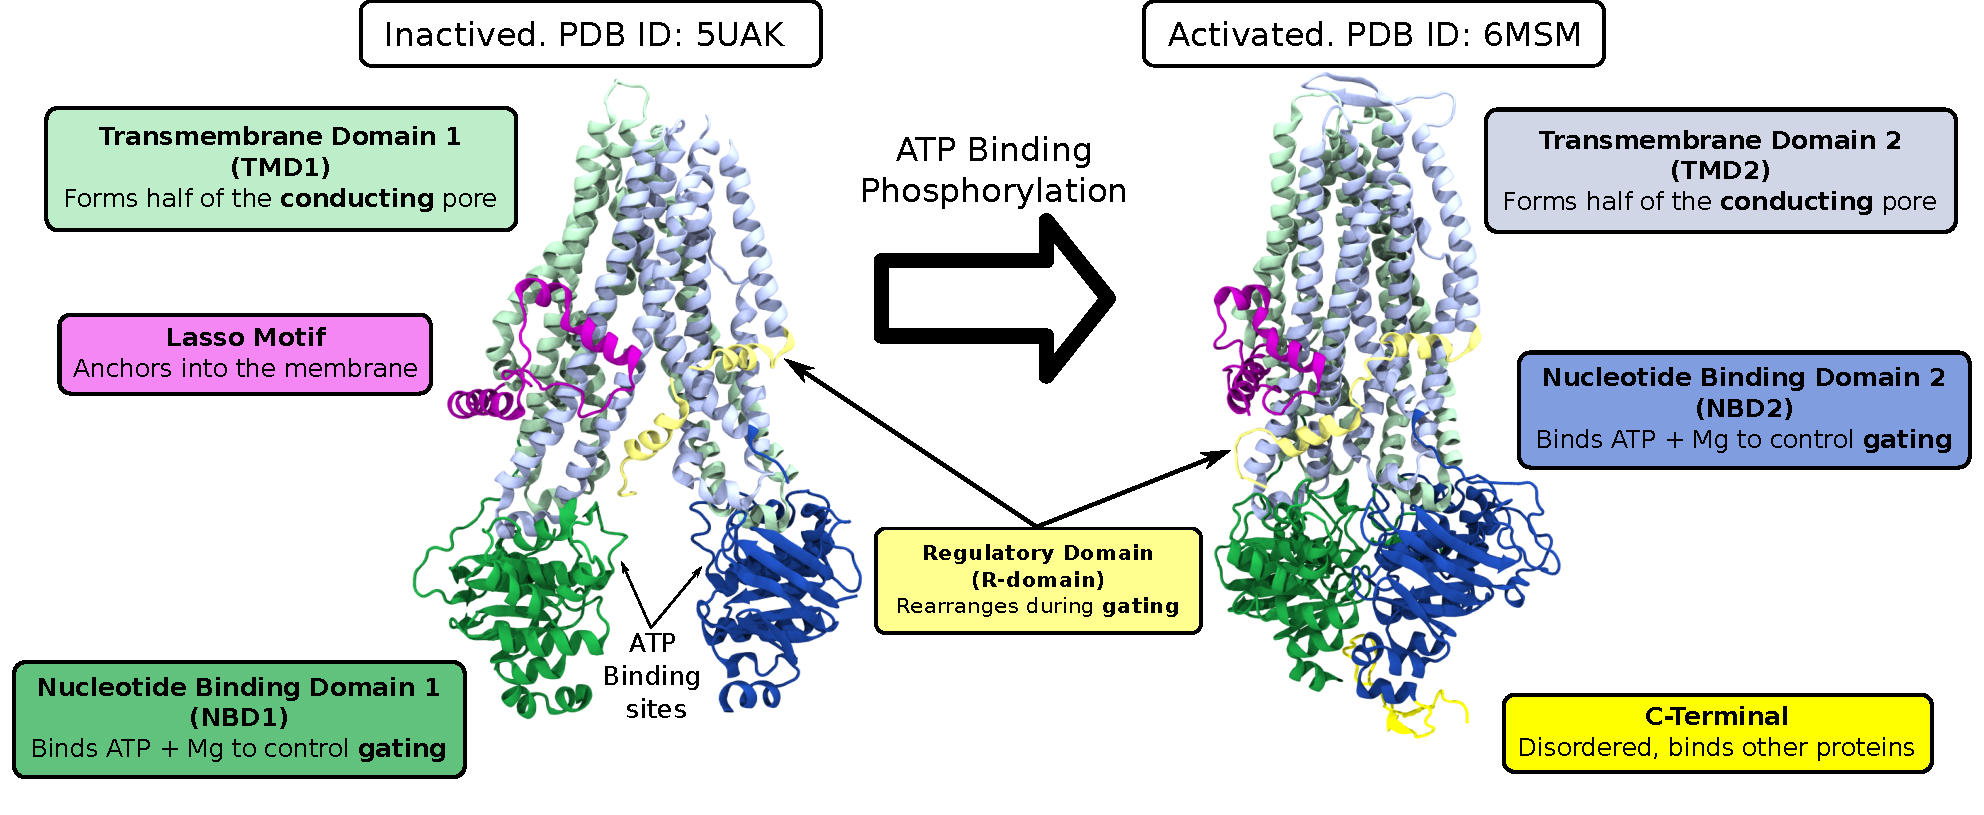
\includegraphics[width=\textwidth]{figures/CFTR_structure.pdf}
	\end{center}
	\label{CFTR_structure_domains}
	\captionsetup{singlelinecheck = false, justification=raggedright}
	\caption[CFTR Structure] {\textbf{CFTR Structure}}{There are currently two resolved human structures. The inactivated state is neither phosphorylated nor bound to ATP. Observe how the NBDs are far apart and the TMDs are not parallel, forcing a constriction which does not allow the passage of ions. By contrast, the activated structure is abound to ATP at both sites, bringing the TMDs into a parallel configuration where they form a pore. There are unresolved questions as to whether CFTR may conduct chloride in this conformation which we will analyse in chapter \ref{chap:opening}.} 
\end{figure}
CFTR is composed of one chain with pseudo-symmetric structure, the protein is well organised into 7 domains \ref{CFTR_structure_domains}. In the order of their primary structure they are: 
\begin{enumerate}
	\item The Lasso motif (AA 1-68). Anchors into the membrane and serves as an interaction hub with protein partners such as syntaxin and filamin which are important in cellular trafficking \cite{cormet-boyaka2002}\cite{naren1998}\cite{thelin2007} as well as WNK1 which plays a role in bicarbonate selectivity \cite{kim2019}.
	\item Transmembrane Domain 1 (TMD1 AA 69-376). This domain forms half of the chloride conducting pore and importantly, in the activated human structure 6MSM forms the extracellular  pore for anion permeation\cite{}.
	\item Nucleotide Binding Domain 1 (NBD1 AA 377-629). One of the ATP binding sites, this domain has a dense concentration of disease causing mutations, including the most common mutation $\Delta F508$ \cite{thehospitalforsickchildren2020}.
	\item Regulatory Domain (R-domain AA 630-855). A disordered domain containing up to 11 phosphorylation sites\cite{mihalyi2020}. In the inactivated conformation a helical segment of this domain wedges between the TMDs. Upon binding of PKA and phosphorylation the wedge relocates to a location just below the R-domain. The identity of this wedge is analysed in detail in chapter \ref{chap:I37R}. The kinetics of this domain is important to the overall function of CFTR. 
	\item Transmembrane Domain 2 (TMD2 AA 856-1168). This domain forms the other half of the chloride conducting pore. There is ongoing controversy over the structure and function of TM8 the function of CFTR \cite{hegedus2022}\cite{liu2019}.
	\item Nucleotide Binding Domain 2 (NBD2 AA 1169 - 1450). Home to the conserved Q-loop, which plays an important role in the binding of ATP in ABC transporters \cite{ivey2020}\cite{zolnerciks2014}\cite{dong2015}.
	\item C-terminus (NBD2 AA 1451 - 1480). 
\end{enumerate}
Transmembrane Domain 1 (TMD1) which forms half of the pore. Nucleotide Binding Domain 1 (NBD1) which binds ATP when the channel is in the open state. The Regulatory domain (R-domain) which, when phosphorylated allows the channel to open. Transmembrane domain 2 (TMD2) which forms the other half of the ion conducting pore. Nucleotide Binding Domain 2 

CFTR belongs to a super family of proteins known as ATP Binding Cassette Transporters,  many of these proteins perform active transport across cell membranes. The substrates they transport can vary, including lipids and drug molecules. Proteins in this family share a common motif known as Nucleotide Binding Domains (NBDs). These domains act as ATPases, accelerating the hydrolysis of ATP. The energy from hydrolysis is then transferred into the protein in order for it to pump its substrate against a concentration gradient. 

\section{CFTR is a Unique ABC Transporter}

\begin{figure}
	\label{ABC_diversity}
	\begin{center}
	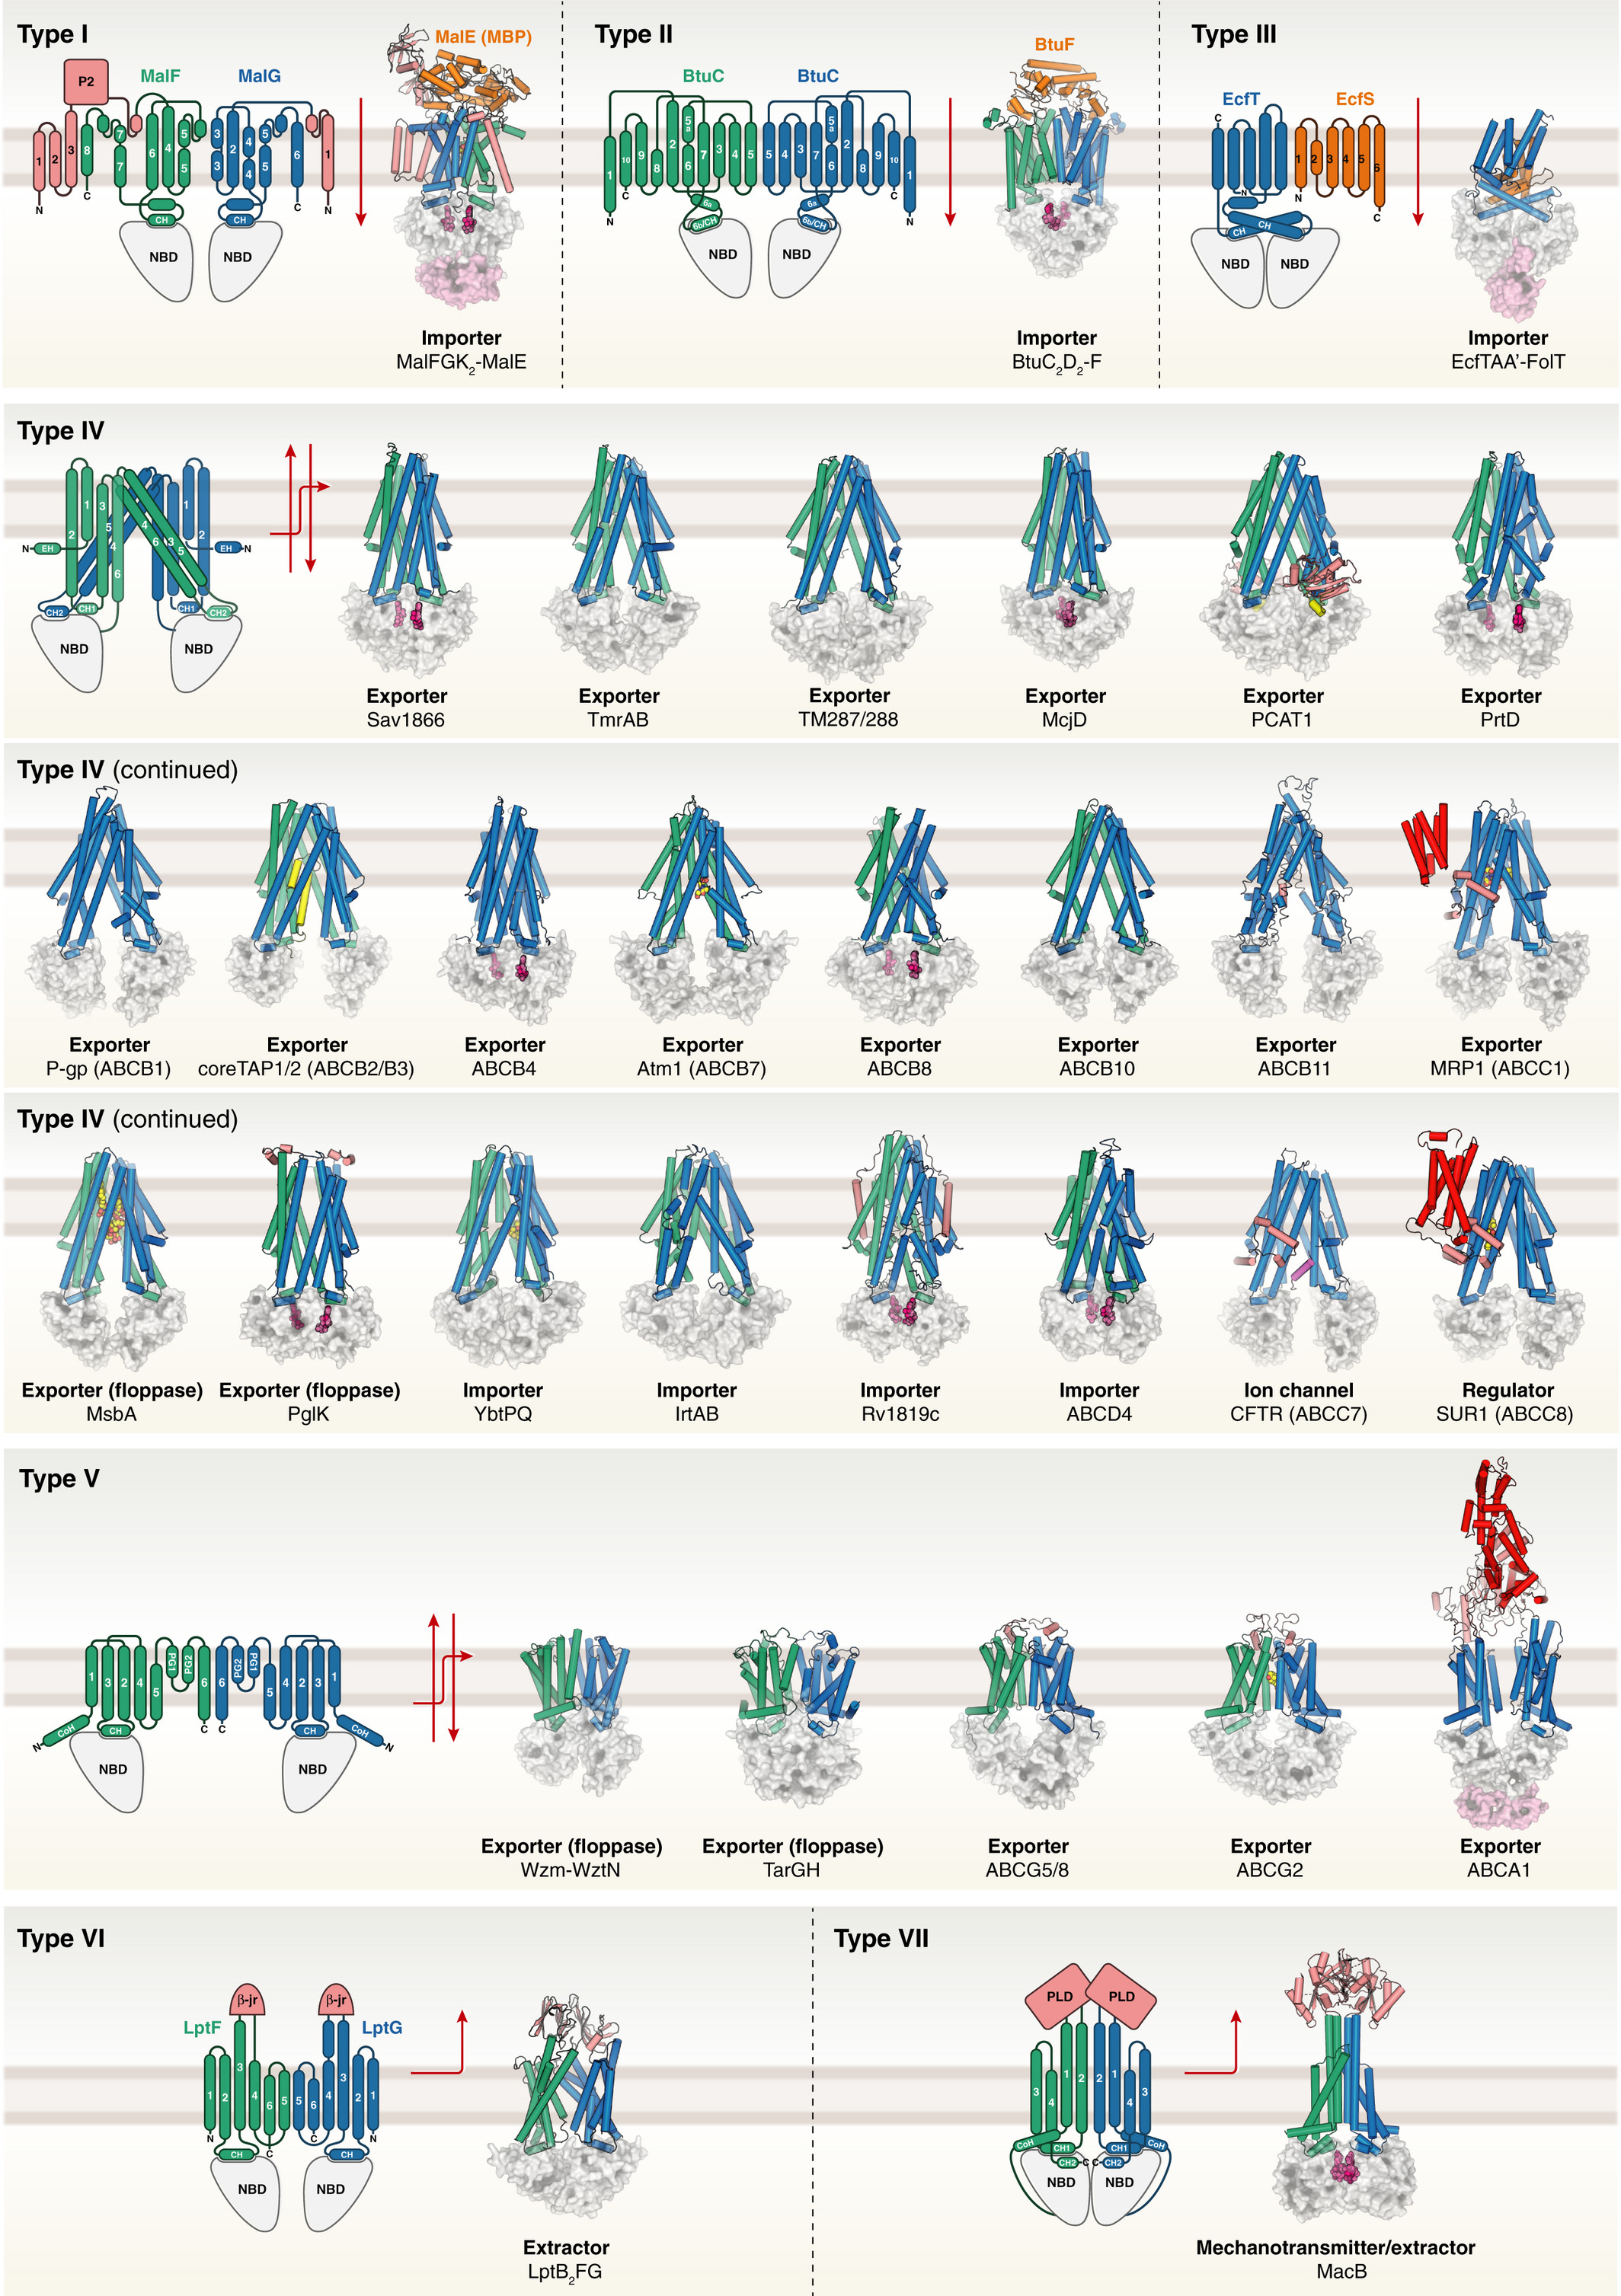
\includegraphics[width=\textwidth]{figures/ABC_classification.jpg}
	\end{center}
	\captionsetup{singlelinecheck = false, justification=raggedright}
	\caption[CFTR Structure] {\textbf{CFTR Structure}}{The structural diversity of ABC transporters. Structures are classified based on the organisation of their TMDs source \cite{thomas2020}.} 
\end{figure}
ATP-Binding Cassette (ABC) transporters are an intriguing super family of proteins. On the whole, they transport substrates by using a combination of phosphorylation energy from ATP hydrolysis. These can be diverse substrates such as lipids or small molecules. Their structural diversity can be seen in figure \ref{ABC_diversity} reflecting their array of functions. 

CFTR is unique, as it is not a transporter, but rather an anion \textit{channel}. The kinetic energy of the ATP is not used to translocate substrate across the membrane but rather simply used in the regulation of the gating cycle. Chloride, bicarbonate and other anions are able to \textit{passively} diffuse through the channel. This evolutionary misappropriation of a transporter to a "leaky channel" is perhaps the reason so many mutations can create a non-functional protein \cite{linsdell2018}.

\section{CFTR classification and structure}

The primary cause of the disease Cystic Fibrosis (CF) is the malfunction of a chloride channel, the Cystic Fibrosis Transmembrane Conductance Regulator (CFTR). This ion channel is a member of the ABCC subfamily of ABC transporters, designated ABCC7. This channel is unique amongst this family because it is not generally considered an active transporter but something of a low conductivity channel or a "weak pump"\cite{linsdell2018}.

CFTR is distinguished by a regulatory region known as the R-domain (residues 645-845) which links NBD1 to TMD2. This region acts to lock the channel in the closed state by wedging itself between the TMDs and dislodging when any one of 3 sites are phosphorylated \cite{mihalyi2020}. In experimentally determined structures of human CFTR the secondary structure of a section of the R-domain but not at high enough resolution to determine the identity of individual side chains \cite{zhang2018}\cite{zhang2016}. Further secondary structure information can be found through experiments with NMR \cite{Baker2007}.

Previous computational studies of CFTR have been used homology models based on the phosphorylated zebra fish protein PDBID:5W81 \cite{zhang2017a}. These have yielded interesting results but the sequence similarity between human and zebra fish CFTR is only 55\% \cite{}. For a protein structure where a single amino acid mutation leads to malfunction, more precision can only help. Additionally, the activity of CFTR modulators is not conserved in mutant zCFTR possibly because it has different kinetics to the human channel \cite{}. In order to do precision medicine we need precision structures. 

An open state of the channel has been proposed by combining both the zebra fish homology model and the fully outward facing conformer of a bacterial ABC transporter Sav1866 \cite{Hoffmann2018}. Although this model has several characteristics expected of the open channel, such as the critical R352-D993 salt bridge, it lacks a salt bridge between R104-E116. In experiments, these residues could be replaced by cysteines and the channel would still function. However, when reducing agents were added to the system the channel lost its ability to open fully. This indicates that in the oxidised environment the C104-C116 cysteines formed a disulfide bridge but its breaking upon exposure to reducing agents caused a loss of function in the channel. This indicates that in the WT channel R104-E116 form a stable salt bridge. 

This salt bridge is clearly visible in the recent cryo-EM structure of ATP-bound human CFTR \cite{zhang2018}.

\section{The Gating Cycle}
The conformational transition from inactive to active differs significantly in CFTR compared to other ABC transporters. The NBDs are largely similar to other to those found in other ABC transporters, they dimerise in what is termed a head to tail configuration so both subunits contact both bound ATP molecules \cite{} See FIGURE. Residue E1371 allows nucleophilic attack on the $\gamma$ phosphate of the ATP bound to Walker B \cite{Stratford2007}. This provides a "kick" to provide the kinetic energy for the opening of the channel CITATION NEEDED. 

\section{Classes of Misfunction to CFTR}
The 360 disease causing mutations to CFTR have been classified into 6 common classes based on the nature of the CF they cause, their reaction to CFTR modulators, and results \textit{in vitro} assays. Ultimately I aim to show that at the atomic level these classes of mutations are less meaningful and as patient specific theratyping evolves these classes will become less relevant, serving as illustrative tools only to communicate at a higher level what is going wrong with the CFTR protein. The canonical classification is as follows:
\begin{itemize}
	\item \textbf{Class I} No functional protein. Under these mutations no protein is transcribed due to either problems with the transcription of mRNA or a premature stop codon truncating protein synthesis early, meaning the resulting peptide is missing key domains. 
	\item \textbf{Class II} Folding defect. These mutations cause the translated peptide to misfold into the incorrect tertiary structure. This can inhibit the protein's journey as it is trafficked to the cell membrane, its function while once it is there or its functional life time at the surface. 
	\item \textbf{Class III} Impaired Gating. Here the mutation inhibits the ability of the protein to transition from the closed to the open state. 
	\item \textbf{Class IV} Decreased Conductance. These mutations cause a barrier in the energy landscape of the CFTR chloride conductance pathway.
	\item \textbf{Class V} Less Protein Expressed.  
	\item \textbf{Class VI} Decreased Lifetime

\end{itemize}

Although useful, in reality this paradigm struggles to reflect the fact that a mutation can belong to multiple categories to different levels due to different modes of pathogenesis. Through our molecular simulations we can see that in reality CFTR modulators are capable of treating several different mutations with very different molecular fingerprints. We will break down this paradigm into more molecular detail in chapter \ref{chap:outlook_review}

FIGURE demonstrates how each of the canonical classes at the molecular level is broken down into many sub classes and a mutation might belong to one of many of these subclasses. Structural biology paradigms and \textit{in silico} modelling can help classify mutations into these different classes. In combination with wet lab assays we can understand which classes of these molecular defects are most effectively treated with specific drug regimens. Our computational microscope is helping choose treatments for patients at the atomic level. 

\section{CFTR Modulators}
Since CF is caused by malfunctions of the channel it makes sense to pursue CFTR as a drug target. Through high throughput \textit{in vitro} screening several (GET NUMBER) compounds have been developed that aim to rescue the function of CFTR. These fall into two classes. Correctors, which aid CFTR to fold into the correct state and potentiators which help the channel reach the fully open state once it has already folded correctly. Emerging evidence suggests that specific genetic defects may be optimally rescued by specific combinations and doses of both correctors and potentiators compounds. Recently, cryo-EM structures of these compounds in their bound state have been released. In addition to several \textit {in vitro} biophysical experiments to determine the precise mechanism of action and binding site of these compounds.

\subsection{Correctors}
The mechanism of action for corrector compounds appears to be to bind to to a pocket between TMH1 and TMH3. Circular dichromism and fluorescence experiments found that an isolated construct of TMH3 and TMH4 were more likely to fold correctly in the presence of corrector compounds. Later cryo-EM structures discovered high resolution electron density in the pocket in the shape of the drug compounds \cite{fiedorczuk2022}. 

In combination this is strong evidence for the precise mechanism of action for corrector compounds. Further work will aid in the creation of new compounds to refine our exploitation of this mechanism.

Mention that there are some interactions between correctors and NBD1.

\subsection{Potentiators}
There is more uncertainty surrounding the mechanism of potentiators drugs. Experiments clearly demonstrate that they act directly on CFTR in order to increase the likelihood that it occupies the open state. They bind to the protein with picomolar affinity. There are are cryo-EM structures which show the drugs bound to the TM8 hinge region \cite{}. \textit {In vitro} experiments suggest at least two membrane facing binding pockets due to the drugs extreme hydrophobicity\cite{}. The location of this second binding site is unknown. The difficulties arise with mutagenesis experiments. The dose-response curves in several studies show that when various sites are mutated the activity of the drug is lowered. This indicates additional binding sites not yet well defined. 

GLPG1837 has not been approved in a clinical setting. \textit {in vitro} experiments suggest that it is more efficacious even though it has lower affinity for CFTR binding (CITATION NEEDED). This would indicate that the highest affinity binding pocket does not produce the greatest modulation. More work is needed to resolve the mechanism which results in the clinical effectiveness of these drugs.  

These drugs are clinically efficacious \cite{VanGoor2014} on several mutants with some curious exceptions like N1303K. I suggest the following mechanism for their action. I suspect a similar analogy exists for the action of the correctors. WT-CFTR exhibits a natural landscape with kinetic barriers in the transition between the closed and open states. A gating class mutation to CFTR will introduce a kinetic barrier in the pathway of this conformational transition. What these drugs do is reduce a barrier in the existing conformational landscape of CFTR. This compensates for the barriers introduced by the mutation. 

This provides a rationale for why it appears possible for diverse range of molecular defects to be treatable by these small molecules. In our work we've found that the atomic nature of the defects introduced by each mutation varies widely, what is interesting is that experiments in \textit{ex vivo} models have shown that these drugs treat a variety of different defects. The classification of classes of defect is outdated, really there are as many classes as there are mutations.


\subsection {Anion Selectivity}
CFTR is weakly selective for specific anions. F337 is the most important amino acid for selectivity. Bicarbonate (HCO$_3^-$ is known to have roughly 26\% the permeability of chloride through the channel. Note that Fluoride has even higher conductance through CFTR, likely due to its small size and high solvation energy (does this indicate hydrated conductance?). WNK1 is known to influence the selectivity of the channel https://www.ncbi.nlm.nih.gov/pmc/articles/PMC6889609/. The permeation of bicarbonate is very important physiologically because if a mutation permeates bicarbonate it means there is a high likelihood the patient will be pancreatic sufficient. 

Compared to cation channels like Gramicidin and KcsA, CFTR is only weakly selective, permeating a large set of annions with varying radii and geometries. Supposedly it is more permeant to lyotropic (low solvation energy annions) rather than cosmotropic anions (high solvation energy annions) indicating that dehydration of the anion is likely during conductance (CITATION NEEDED). The radius of hydrated chloride ions is 1.7A\cite{yang2002} so even with this larger pore partial dehydration must take place. 

\section{Addressing Controversies Surrounding the Structure of CFTR}
The most recent structure of human CFTR in a phosphorylated environment has some interesting features which have lead to some controversies in the literature. After spending significant time researching them I have conducted an extensive literature review in order to learn more about of these concerns. The released structure of activated, human CFTR has two features that have caused some in the CF field to suggest issues with this structure. Firstly, this structure is not sufficiently open to conduct chloride ions. Chloride ions have a diameter of 1.7$\AA$ while the structure has a constriction of 1.1$\AA$\cite{Zhang2018}. So, there must be some level of conformational changes, even if chloride were to move through the channel completely dehydrated. This becomes even more of an issue when considers the experimental evidence where much larger anionic species such as bicarbonate and glutathione were shown to permeate through the channel\cite{kogan2003}. This suggests that there is a much larger conformation which has not been observed experimentally or in simulations. This was the motivation for chapter \ref{chap:opening} of this thesis. Some studies have been performed in order to study the possible permeation paths of chloride but they have not addressed the pressing question of how larger ions might permeate the channel. Bicarbonate in particular is of great physiological importance as there is a high correlation between the channel's ability to permeate bicarbonate and the pancreatic sufficiency of a patient carrying the mutation. In light of this, structural knowledge of a fully open conformation of CFTR is critical to a personalised approach to the treatment of CFTR.

The second and harder to resolve controversy concern the role of TM8. This transmembrane helix has an unusual bend in the middle of the plasma membrane. This is not something seen before in ABC transporters of this type. So it has led to some open questions as to how this bend might contribute to the function of the channel \textit{or} how it might be an artifact of the imaging process. For the former case, the structural biologists in the Chen lab proposed a mechanism whereby the upper hinge of TM8 swings 55$^o$ during the transition to the open state. This mechanism would give justification of the pathogenesis of certain mutaions such as L927P. 

The arguments for the bend in the helix appear to be unphysical. In cryoEM structures, we can observe that the bent conformation is stabilised by salt bridges R347-D924 and E873-R933. The former bond has been well studied experimentally and was expected in the 3d structure. Additionally, all hydrogen bonds along the in the bent helix are . Been observed to be stable in MD \cite{corradi2018} .  is energetically stable.

However, there are still some unanswered questions for the discrepancy between the solved human and solved chicken structures. Certain salt bridges are not present in the latter structure and so single channel electrophysiology experiments may be able to resolve these issues. For example, in 6MSM, the human structure of CFTR there is a salt bridge between amino acids 933 and D873 which is not present in the chCFTR structures. This bond is also present in the zCFTR structure 5W81. If a charge swapped mutant such as R933E/E873R restores WT-like gating behaviour to the channel it would be  strong evidence for the unwound conformation of TM8. 

The two proposed conformations also have vastly different ion permeation pathways, and so blockers engineered to target one conformatoin over the other would also go a long way to answering these questions. The available evidence strongly favors the R334 pathway between TM1 and TM6. Such as experiments to  demonstrate the blockage of current with zinc have shown that mutations to R334 strongly suggest that chloride permeates along this route. Additionally, trhere are several disease causing mutations in the region surrounding R334, such as R334W, R117H, E116K, D110H, I336K\cite{cftr2}. This permeation route also explains the rationale behind the gain of function mutation F337A \cite{}. Determining which model is correct has wide implications for creating the next generation of mutation targeted potentiator class drugs.

A study assessing the accuracy of Alphafold's predictions of transmembrane protein structures found an intersting result. When alphafold made predictions that involved the use of templates it predicts the unwound conformation of TM8. On the other hand, when templates are removed from alphafolds predictions it predicts a straight TM8 conformation, very similar to that found in chCFTR. The authors of this study suggested the reason for the discrepancy was due to the use of detergents in the deteremination of the structure of hCFTR. However, careful reading of cryo-EM literature reveals no examples where the use of detergents has resulted in such drastic conformational changes. One of the few examples where both detergents and native-like nanodisks were used to determine the structure of a protein are the determinations of the structure of TRPV1. These studies revealed no difference to the backbone helices but did suggest important information about the the importrance of different interactions with lipids. A lot of work has been performed in order to create detergents which reflect a native lipid environment and these are the species that were used in . 

The authors of the chCFTR paper suggested that the different expression systems used in the two studies could be the reason for the discrepancy between the two systems, due it their different post translational processing apparatus. Although both groups used mammalian cell lines the chCFTR paper used hamster? cells \cite{aleksandrov2015} and the Chen lab used HEK293S cells. The chicken structure underwent significant mutations in order to be locked open and crystallised. The regulatory insertion was deleted, Many hydrophobic amino acids were introduced into NBD1 in order to aid in the purification of the protein. 

Figure \ref{} shows the large diversity of structures in type IV ABC transporters, many of which also exhibit bends within transmembrane helices\cite{thomas2020}. 
>>>>>>> dfa8ae7c815116d94d0aada27fa917fd6409538a

\section{Patient Derived Organoids}
The basic unit of living things are cells. In the medical field there is growing capability to discern the functioning of an individual patient's cells. In the field of Cystic Fibrosis Medical Research a recent breakthrough has been to take samples from the epithelium of patients with the disease and grow those samples into tissues which mimic the function of the entire organ\cite{depoel2020}. This is possible in the epithelium due to a population of adult stem cells which maintain the ability to differentiate into a variety of cell types (a property known as pluripotency). 

Adult stem cells in the epithelium are preferable because other sources of stem cells such as induced pluripotent stem cells (iPSCs) require complex, time consuming protocols to grow into fully developed organoids. 

In the case of CF this technology allows the construction of a scalable, patient specific platform where a patient's own tissues can be tested to determine the best treatment for them. These pre-clinical models will allow more patients in the heterogeneous set of disease causing mutations to access modulators. 

Forskolin Induced Swelling (FIS) assays have been used to characterise the patient specific response of a patient's organoids to a drug regimen \cite{dekkers2013}. 


One limitation of these organoid platforms is the lack of an inflammatory response since no immune cells are present in the tissue culture. 


%

%=======================================================================================%
\chapter{Molecular Dynamics and Functional Characterization of I37R-CFTR Lasso Mutation Provide Insights into Channel Gating Activity}
\label{chap:I37R}
\section*{\centering Abstract} 
Characterization of I37R, a mutation located in the lasso motif of the CFTR chloride channel, was conducted by theratyping several CFTR modulators from both potentiator and corrector classes. Intestinal current measurements in rectal biopsies, forskolin-induced swelling (FIS) in intestinal organoids, and short circuit current measurements in organoid-derived monolayers from an individual with I37R/Fidel CFTR genotype demonstrated that the I37R-CFTR results in a residual function defect amenable to treatment with potentiators and type III, but not type I, correctors. Molecular dynamics of I37R using an extended model of the phosphorylated, ATP-bound human CFTR identified an altered lasso motif conformation which results in an unfavorable strengthening of the interactions between the lasso motif, the regulatory (R) domain, and the transmembrane domain 2 (TMD2). Structural and functional characterization of the I37R-CFTR mutation increases understanding of CFTR channel regulation and provides a potential pathway to expand drug access to CF patients with ultra-rare genotypes.

%=======================================================================================%
\chapter{Molecular Dynamics and Theratyping in Airway and Gut Organoids Reveal R352Q-CFTR Conductance Defect}
\label{chap:R352Q}
\chapquote{Cells have a mind of their own-Shafagh Waters} {}

\section*{\centering Abstract} 
A significant challenge to making targeted CFTR modulator therapies accessible to all individuals with cystic fibrosis (CF) are many mutations in the CFTR gene that can cause CF, most of which remain uncharacterized. Here, we characterized the structural and functional defects of the rare CFTR mutation R352Q – with potential role contributing to intrapore chloride ion permeation – in patient-derived cell models of the airway and gut. CFTR function in differentiated nasal epithelial cultures and matched intestinal organoids was assessed using ion transport assay and forskolin-induced swelling (FIS) assay respectively. CFTR potentiators (VX-770, GLPG1837 and VX-445) and correctors (VX-809, VX-445 +/- VX-661) were tested.  Data from R352Q-CFTR were compared to that of twenty participants with mutations with known impact on CFTR function. R352Q-CFTR has residual CFTR function which was restored to functional CFTR activity by CFTR potentiators but not the corrector. Molecular dynamics (MD) simulations of R352Q-CFTR were carried out which indicated the presence of a chloride conductance defect, with little evidence supporting a gating defect. The combination approach of in vitro patient-derived cell models and in silico MD simulations to characterize rare CFTR mutations can improve the specificity and sensitivity of modulator response predictions and aid in their translational use for CF precision medicine.

%=======================================================================================%
\chapter{Unique S945L-CFTR defect Restored by CFTR Modulator Co-Therapy In Vitro Correlates with In Vivo Biomarkers Post-Therapy}
\chapquote{Soon you'll realise you're two days from anywhere} {-David Goodwin}
\label{chap:s945l}

%=======================================================================================%
\chapter{Resolving a Conducting Conformation of CFTR Using Free Energy Calculations}
\label{chap:opening}
\chapquote{} {}
ABSTRACT 
Understanding how CFTR conducts ions is critical to ongoing drug discovery efforts to treat Cystic Fibrosis. Existing structures of CFTR  raise unresolved qustions as to how CFTR conducts ions as they exhibit a constriction smaller than the ions themselves. This indicates that there must be some level of conformational change for ions to pass through this structure. Here we present innovative simulation techniques combining simple numerical techniques and new advances in free energy calculations to resolve the full conduction pathway in CFTR. We hope that the techniques and philosophy in this chapter will be refined and applied to other complex protein systems of physiological relevance. 
\newline

\section{Discussion}

The present study diverges in an important way from existing free energy calculations which investigate protein conformational changes in the literature. Present studies have focussed on recreating intermediate free energy landscapes between \textit{known} endpoints \cite{lev2020, bergh2021}. Such approaches are critical to the developement of molecular techniques in order to understand the energetics and kinetics of molecular machines. However, these studies are inherently limited to the availability of high quality experimental 3d structures. Protein forcefields may have their issues but they are now of sufficient quality that they can now be used, alongside considerable computer power to investigate parts of the conformational landscape which have critical functional roles but are not covered by experimental structures. This is akin to the developement of an unsupervised vs. supervised machine learning algorithms. Each approach is powerful but has its own domain of applicability and drawbacks. 

As shown by the results in the present study the difficulty in converging a free energy landscape with collective variables derived \textit {ab initio} from long classical MD simulations can be difficult as the CVs are very likely going to be suboptimal. Machine learning techniques, more sophisticated than the simple PCA algorithm used here would likely do a much better job of choosing quickly converging CVs. 

%=======================================================================================%
\chapter{Concluding Remarks: Where next for Molecular Studies of CFTR.}
\label{chap:conclusion}
\chapquote {We have more problems than hands. - Eduardo Perozo}{}

As figure \ref{CF_life_expectancy} demonstrates, basic science discoveries concerning CF have had a direct effect on the life expectancy of patients. This proves the utility . The work in this thesis is a small example of how abstract physical models, such as those outlined in \ref{chap:methods}, can be applied to help real patients in a community such as allowing patients in Sydney Children's hospital to access medications which could add decades to their life span. We are entering an exciting era of biophysical research where advances in theoretical methods, computing power and experimental techniques are beginning to drive advances in each other at a frenetic pace. An example can be seen in the development of Alphafold. The maturation of cryoEM allowed the discovery of new protein folds which Alphafold's machine learning algorithms could then learn from. Now that the algorithm had these folds in hand it could predict entire proteomes. This now means that structural biologists can use the predictions of alphafold to solve even more structures more quickly. Eventually, more and more of the experimental work currently involved in biology will move onto the silicon chip, while experimental techniques will advance in other areas. Similarly, the theoretical model argued for in this thesis will eventually allow for patient assessments to be made \textit{in silico}

The preceeding chapters have given technical and molecular details about how Cystic Fibrosis is caused by rare mutations and further demonstrated that these mutations may be treated by existing small molecule drugs. The unique molecular fingerprint of each mutation indicates that in order to deliver better outcomes to patients a more personalised approach is necessary to the choice of medication. For this personalisation to be possible there are some basic questions about CFTRs structure and function that remain to be answered. Some of these questions simulations are uniquely placed to answer. 

Additionally, I'd like to propose a theoretical model for the action of these drugs which would appear to suggest that more patients should be given access to existing medications and inform the design of future generations of CFTR modulators. 

As such, the areas which deserve the most attention for molecular studies of CFTR are to address the controversies surrounding its structure and elucidate the action of drug binding. Together these will allow a clearer understanding of CFTRs function in health and misfunction in disease, enableing more targetted drug development. Current generation modulators have been identified using high throughput screening, the new generation of high computational power, artificial intelligence and structural data will allow a more targetted, perhaps even mutation specific approach to the design of new modulators.

\section{Addressing Controversies Surrounding the Structure of CFTR}
The most recent structure of human CFTR in a phosphorylated environment has some interesting features which have lead to some controversies in the literature. After spending significant time researching them I have conducted an extensive literature review in order to learn more about of these concerns. The released structure of activated, human CFTR has two features that have caused some in the CF field to suggest issues with this structure. Firstly, this structure is not sufficiently open to conduct chloride ions. Chloride ions have a diameter of 1.7$\AA$ while the structure has a constriction of 1.1$\AA$\cite{Zhang2018}. So, there must be some level of conformational changes, even if chloride were to move through the channel completely dehydrated. This becomes even more of an issue when considers the experimental evidence where much larger anionic species such as bicarbonate and glutathione were shown to permeate through the channel\cite{kogan2003}. This suggests that there is a much larger conformation which has not been observed experimentally or in simulations. This was the motivation for chapter \ref{chap:opening} of this thesis. Some studies have been performed in order to study the possible permeation paths of chloride but they have not addressed the pressing question of how larger ions might permeate the channel. Bicarbonate in particular is of great physiological importance as there is a high correlation between the channel's ability to permeate bicarbonate and the pancreatic sufficiency of a patient carrying the mutation. In light of this, structural knowledge of a fully open conformation of CFTR is critical to a personalised approach to the treatment of CFTR.

The second and harder to resolve controversy concern the role of TM8. This transmembrane helix has an unusual bend in the middle of the plasma membrane. This is not something seen before in ABC transporters of this type. So it has led to some open questions as to how this bend might contribute to the function of the channel \textit{or} how it might be an artifact of the imaging process. For the former case, the structural biologists in the Chen lab proposed a mechanism whereby the upper hinge of TM8 swings 55$^o$ during the transition to the open state. This mechanism would give justification of the pathogenesis of certain mutaions such as L927P. 

The arguments for the bend in the helix appear to be unphysical. In cryoEM structures, we can observe that the bent conformation is stabilised by salt bridges R347-D924 and E873-R933. The former bond has been well studied experimentally and was expected in the 3d structure. Additionally, all hydrogen bonds along the in the bent helix are . Been observed to be stable in MD \cite{corradi2018} .  is energetically stable.

However, there are still some unanswered questions for the discrepancy between the solved human and solved chicken structures. Certain salt bridges are not present in the latter structure and so single channel electrophysiology experiments may be able to resolve these issues. For example, in 6MSM, the human structure of CFTR there is a salt bridge between amino acids 933 and D873 which is not present in the chCFTR structures. This bond is also present in the zCFTR structure 5W81. If a charge swapped mutant such as R933E/E873R restores WT-like gating behaviour to the channel it would be  strong evidence for the unwound conformation of TM8. 

The two proposed conformations also have vastly different ion permeation pathways, and so blockers engineered to target one conformatoin over the other would also go a long way to answering these questions. The available evidence strongly favors the R334 pathway between TM1 and TM6. Such as experiments to  demonstrate the blockage of current with zinc have shown that mutations to R334 strongly suggest that chloride permeates along this route. Additionally, trhere are several disease causing mutations in the region surrounding R334, such as R334W, R117H, E116K, D110H, I336K\cite{cftr2}. This permeation route also explains the rationale behind the gain of function mutation F337A \cite{}. Determining which model is correct has wide implications for creating the next generation of mutation targeted potentiator class drugs.

Mutagenesis studies of the outer pore would strongly support the Chen structure over the chicken streucture. In particular, Paul Linsdell performed very careful experiments to measure blockage chloride blockage and found that several residues play an important role in the permeation of chloride in the outer pore. In the chicken structure these residues are occluded and far from the chloride permeation pathway. However, in the Chen structure they appear to play an important role in the permeation of chloride. This will be discussed in detail in \ref{chap:opening}.

A study assessing the accuracy of Alphafold's predictions of transmembrane protein structures found an intersting result. When alphafold made predictions that involved the use of templates it predicts the unwound conformation of TM8. On the other hand, when templates are removed from alphafolds predictions it predicts a straight TM8 conformation, very similar to that found in chCFTR. The authors of this study suggested the reason for the discrepancy was due to the use of detergents in the deteremination of the structure of hCFTR. However, careful reading of cryo-EM literature reveals no examples where the use of detergents has resulted in such drastic conformational changes. One of the few examples where both detergents and native-like nanodisks were used to determine the structure of a protein are the determinations of the structure of TRPV1. These studies revealed no difference to the backbone helices but did suggest important information about the importance of different interactions with lipids. A lot of work has been performed in order to create detergents which reflect a native lipid environment and these are the species that were used in . 

The authors of the chCFTR paper suggested that the different expression systems used in the two studies could be the reason for the discrepancy between the two systems, due it their different post translational processing apparatus. Although both groups used mammalian cell lines the chCFTR paper used hamster? cells \cite{aleksandrov2015} and the Chen lab used HEK293S cells. The chicken structure also underwent significant mutations in order to be locked open and imaged. The regulatory insertion was deleted in order to aid in the purification of the protein. 

Figure \ref{} shows the large diversity of structures in type IV ABC transporters, many of which also exhibit bends within transmembrane helices\cite{thomas2020}. Although none of these structures exhibit such a bend in TM8 specifically, the 

\ref{negoda2019} gives strong evidence that TM8 must line the conduction pore. Due to its proximity to F337 and other pore lining amino acids. This is more consistent with the Chen structure than the chicken structure where 337 is far from the conduction pore.

\section{A Physics Motivated Model for the Molecular Modulation of Mutant CFTR }
In chapter \ref{chap:I37R}, \ref{chap:R352Q}, \ref{chap:S945L} and \ref{chap:opening} we have analysed a disease causing mutation in detail in order to understand \textit{how} they cause CFTR to misfunction. What we have found is a large diversity of molecular phenotypes which may cause disease. What is thus remarkable is that the \textit{in vitro} component of these papers all demonstrate that these mutations are responding to the same drugs, albeit with differing efficacies.



The above model in figure \ref{drug_action_model} gives a rational, physical basis for the wide range of molecular phenotypes that CFTR modulators appear capable of treating. This same model would appear to argue that for most missense mutations we would expect them to respond to some sort of CFTR modulator.

\section{A Physics Motivated Approach to Personalised Medicine}

The success of the mutation specific approach to personalised medicine used here should be considered when studying other monogenic diseases such as Muscular  Dystrophy, Sickle Cell Anemia and Huntington's disease \cite{}. 

In recent years there have been a slew of rare CF-causing genotypes discovered in populations with low rates of Cystic Fibrosis compared to Caucasians. These genotypes from Asia and the Middle East are often ultra-rare leading to poor outcomes for these patients, particular lb when local health care is sub standard \cite{}. 

The ongoing discovery of rare mutations highlights the importance of this personalised approach to the treatment of CF. The process for developing potentiator class drugs was by studying the G551D mutation. Drugs that were found to restore function for this rare mutation are now widely used by sufferers of cystic fibrosis \cite{}. The study of rare mutations N1303K which currently do not respond to drugs may lead to the discovery of more effective compounds to treat cystic fibrosis such as. Thus, the approach to the treatment of Cystic Fibrosis is intersectional, as more rare mutations are discovered and treated the better the outcomes for all patients with Cystic Fibrosis will be. Each rare mutation sheds light on the function of CFTR and lets us understand and treat the root cause of the disease better.


\definecolor{codegreen}{rgb}{0,0.6,0}
\definecolor{codegray}{rgb}{0.5,0.5,0.5}
\definecolor{codepurple}{rgb}{0.58,0,0.82}
\definecolor{codeorange}{rgb}{0.98,0.6,0.01}
\definecolor{codeorange2}{rgb}{1.0,0.5,0.0}
\definecolor{backcolour}{rgb}{0.95,0.95,0.92}

\lstdefinestyle{customTCL}{
    backgroundcolor=\color{backcolour},   
    commentstyle=\color{codegreen},
    keywordstyle=\color{blue},
    numberstyle=\tiny\color{codegray},
    stringstyle=\color{codeorange},
    basicstyle=\footnotesize,
    breakatwhitespace=false,
    language=tcl, 
    breaklines=true,                 
    captionpos=b,                    
    keepspaces=true,                 
    numbers=left,                    
    numbersep=5pt,                  
    showspaces=false,                
    showstringspaces=false,
    showtabs=false,                  
    tabsize=4
}

\lstdefinestyle{customF90}{
    backgroundcolor=\color{backcolour},   
    commentstyle=\color{codegreen},
    keywordstyle=\color{blue},
    numberstyle=\tiny\color{codegray},
    stringstyle=\color{codeorange},
    basicstyle=\footnotesize,
    breakatwhitespace=false,
    language=fortran, 
    morekeywords={*,getarg},
    breaklines=true,                 
    captionpos=b,                    
    keepspaces=true,                 
    numbers=left,                    
    numbersep=5pt,                  
    showspaces=false,                
    showstringspaces=false,
    showtabs=false,                  
    tabsize=4
}

\lstdefinestyle{customPython}{
    backgroundcolor=\color{backcolour},   
    commentstyle=\color{blue},
    keywordstyle=\color{codeorange2},
    numberstyle=\tiny\color{codegray},
    stringstyle=\color{codegreen},
    basicstyle=\footnotesize,
    breakatwhitespace=false,
    language=Python, 
    breaklines=true,                 
    captionpos=b,                    
    keepspaces=true,                 
    numbers=left,                    
    numbersep=5pt,                  
    showspaces=false,                
    showstringspaces=false,
    showtabs=false,                  
    tabsize=4
}

\newpage
%\addcontentsline{toc}{chapter}{\hyperref[apx:charges]{Appendix}}
\appendix



%%%%%%%%%%%%%%%%%%%%%%%
%% Bibliography      %%
%%%%%%%%%%%%%%%%%%%%%%%
\medskip
%\bibliographystyle{IEEEtran}
\addcontentsline{toc}{section}{References}
\printbibliography[heading=bibintoc]

%%%%%%%%%%%%%%%%%%%%%%%
%% Last Quote        %%
%%%%%%%%%%%%%%%%%%%%%%%

\clearpage
\thispagestyle{empty}
\vspace*{2.0in}
%\chapquote{``Nothing ventured, nothing gained."}{}


\end{document}
